\chapter{A Bayesian Spatio-temporal Multisource Air Pollution Exposure Model for the UK}
\section{Abstract}
\textbf{Background and aim:} New 2021 WHO Global Air Quality Guideline levels follow mounting evidence of premature deaths from air pollution exposure, give rise to an increased need for high-quality air pollution modelling strategies. Currently, many areas of the UK exceed the recommended annual PM$_{2.5}$ level of 10 $\mu$g/cm3; however, ground monitoring stations for PM$_{2.5}$ remain sparse. The aim of this study is to produce a 1km x 1km monthly-estimated PM$_{2.5}$ exposure map for the UK between 2005-2020, from AURN ground monitored data, the Pollution Climate Mapping model, and corrected satellite-derived Aerosol Optical Depth, with additional climate covariates from the HadUK-Grid.

\textbf{Methods:} Taking a Bayesian hierarchical approach, the model tackles firstly the misalignment issue from using multi-source data by fitting a spatio-temporal geostatistical model at the ground monitoring site locations. Then a Gaussian process-based approach is used to predict PM$_{2.5}$ across the regions where AOD is available. The usual global stationarity assumption is restrictive for this purpose, so a new regionally-stationary approach has been considered. Finally, interpolation methods, for areas with missing AOD data, will be compared to formulate a complete exposure model.

\textbf{Results:} Preliminary results from a locally-stationary Greater London model display clear spatial variability in ground monitored PM2.5, with different trends identified across site types; as well as a moderate non-linear relationship with temperature humidity and precipitation, creating an overall seasonality trend. The validation of the model via cross-validation technique is currently ongoing.

\textbf{Conclusions:} This model will be used to quantify the effects of air pollution exposure on mental health outcomes in the UK Biobank cohort. Through the use of a Bayesian approach, measurement and modelling uncertainties can be propagated from the exposure model to the mental health effect model.

\section{Background and Review}

\subsection{Air Pollution Monitoring} \label{Section:Air Poll}
%Air pollution is a problem lol, even hippocrates knew this
Since the era of Hippocrates, poor air quality has been recognised as a threat to human health, with speculation of negative health effects as early as 400 BC and documented initial emission regulations dating back to 1273 AD England \cite{Fowler2020AQuality}. Many historical sources attribute Robert Angus Smith as the \textbf{founder} of the \textit{"first multisite, multipollutant measurements"} \citep{Fowler2020AQuality} with his initial findings documented in \textit{'Air and rain: the beginnings of chemical climatology'} \cite{Smith1872AirClimatology} for \emph{`ammonia, nitrate, albuminoid nitrogen, oxidizable organic matter [...], acidity, sulphate and chloride in bulk precipitation.'} \citep{Gorham1982RobertJSTOR}. Historically, the primary source of \textbf{meteorological measurements and} pollution concentrations for exposure assessment has been from fixed weather monitoring stations and pollution sensors, but increasingly the use of alternative \textbf{methods and estimates} has been implemented to allow for higher resolution, more accurate, and more complete estimates \textbf{\citep{Baxter2013ExposureRecommendations}}.

The landscape of air pollution monitoring is continuously changing; with advancements in the understanding of pollutants, the technology of measurement equipment, and also the ever-changing global make-up and, therefore, priorities of pollutant monitoring and control. Modern perspectives consider the so-called classical pollutants, identified for their \emph{`relation to critical health outcomes'} \citep{WorldHealthOrganization2021WHOMonoxide}, see Table \ref{table:2}.

\begin{table}[h!]
\centering
\begin{adjustbox}{width=1\textwidth}
\begin{tabular}{c c c} 
 Pollutant & & Main UK Sources \citep{UKGovernment2019Clean2019} \\ [0.5ex] 
 \hline
  Particulate Matter & PM\textsubscript{2.5}, PM\textsubscript{10} & Domestic and Industrial Combustion, Road Transport, Solvent Use, Industrial Processes \label{pm2.5source}   \\ 
  Nitrogen Dioxide & NO\textsubscript{2} & Road Transport, Energy Generation, Industrial Combustion, Other Transport \\
  Carbon Monoxide & CO & Domestic and Industrial Combustion, Road Transport   \\ 
  Sulphur Dioxide & SO\textsubscript{2} & Energy Generation, Industrial and Domestic Combustion  \\ 
  Ozone & O\textsubscript{3} & Formed through a reaction between other pollutants and UV  \\ [0.5ex] 
 \hline
\end{tabular}
\end{adjustbox}
\caption{Current Global Classical Pollutants as identified by the World Health Organisation \citep{WorldHealthOrganization2021WHOMonoxide}}
\label{table:2}
\end{table}

Particulate matter is the primary consideration for this project due to a multitude of reasons, from the source of the pollutant to it's constituent parts to the impact it has on human health. First, we consider the range of the main sources of particulate matter within the UK (Table \ref{table:2}), which capture a host of both industrial, commercial and domestic activities. Additionally, background rural concentrations of particulate matter have been evidenced to contribute significantly to the overall mass of the pollutant across the UK \citep{DepartmentforEnvironmentFoodRuralAffairs2021Environment2021}, creating an interesting spatial dichotomy between concentrations in rural and urban areas of the UK. Another interesting source of particulate matter in the UK, is the migration of air particles arriving from mainland Europe \citep{Malcolm2000ModellingUK, Abdalmogith2006IntercomparisonModel,Vieno2014TheUK}, known as secondary sources of particulate matter or inorganic particles. These trajectories primarily transport fine particulate matter (PM$_{2.5}$) due to size and their ability to be transported by air particles over long distances \textbf{aerosolibility???} \citep{Vieno2014TheUK}. 

Another important feature of particulate matter, that also differentiates it from gaseous pollutants (e.g. NO\textsubscript{2}, SO\textsubscript{2}), is its broad definition, commonly defined as \emph{`condensed phase solid or liquid particles suspended in the atmosphere'} \citep{AirQualityExpertGroup2012FineKingdom}, which can capture a range of different particle types. The Air Quality Expert Group has identified the principle components of particulate matter and separates them into two categories: primary and secondary \citep{AirQualityExpertGroup2005ParticulateSummary}. Primary components include: sodium chloride (NaCl), elemental or black carbon, organic carbon, trace metals, and mineral dust. Secondary components are from chemical reactions within the atmosphere and include sulphate, nitrate, water, and organic carbon, which come from reactions with Sodium Dioxide (SO\textsubscript{2}), Nitrogen Oxides (NO\textsubscript{x}), Ammonia (NH\textsubscript{3}) and Volatile Organic Compounds (VOCs). 
Particulate matter is further classified into particle size: PM$_{10}$ are \textit{coarse} particles less than or equal to 10 $\mu$m in diameter; PM$_{10}$ are \textit{fine} particles less than or equal to 2.5 $\mu$m in diameter; and occasionally and more increasingly, PM$_{0.1}$ or \textit{ultrafine} particles less than or equal to 0.1 $\mu$m in diameter are considered. There is a lot of literature investigating the negative health effects of both PM$_{10}$ and PM$_{2.5}$ \citep{Harrison2010SizeStudies}, but the general scientific consensus is that finer particles have a more significant association with adverse health affects \cite[p.9-13]{AirQualityExpertGroup2012FineKingdom}. Many studies have investigated the mechanistic pathways for this effect of PM$_{2.5}$ on human health, including via the respiratory system and lungs \citep{Pinkerton2000DistributionLung}, through inflammatory responses or oxidative stress \citep{Brook2008CardiovascularPollution}, and through invasion into the bloodstream \citep{Manisalidis2020EnvironmentalReview}.

Another informative factor of choosing to study PM$_{2.5}$ comes from looking at global compliance with the 2021 WHO Recommended Annual AQC level and interim targets \ref{table:1}. Following a recent report from IQAir \citep{IQAir2021WorldReport}, it can be seen that the UK is continuing to consistently exceed these guidelines for PM$_{2.5}$ and underperform compared to other developed nations, such as Canada, Norway, New Zealand, Sweden and Australia.

\subsubsection{Ground Monitoring Approaches}
The primary source of air pollution data for air quality and exposure modelling has historically been from ground monitoring stations, with evidence showing a rapid increase in global density of ground monitoring networks and stations \citep{Carvalho2016TheMonitoring}. The UK has led the way in introducing national air quality monitoring networks, first implementing 1200 monitoring sites for black smoke and sulphur dioxide in 1961 \citep{DepartmentforEnvironmentBriefHistory}. Since then there has been a shift in the pollutants being measured and the nature of monitoring networks, to give around 300 current air pollution monitoring sites as part of the UK national monitoring network \citep{DepartmentforEnvironmentMonitoringUK}. Automatic monitoring stations represent the most commonly used monitoring type, with hourly pollutant concentrations being taken across the UK, compared to non-automatic monitoring where measurements are less conwistently taken.

In a 2017 review by Gerard Hoek \citep{Hoek2017MethodsPollutants}, the three major methods of using ground monitored data for exposure modelling are explored: nearest station measurements, inter-station averages, and interpolation methods, see Figure \ref{fig:monitormethods}. Studies such as \cite{Ostro2010Long-termStudy} and \cite{Dockery1993AnCities} crudely take the measured value at the nearest monitoring station to be the estimated concentration at a particular point, see Figure \ref{fig:nearest}. A more sophisticated and accurate approach is through the k-nearest neighbour approach, where the average of the k nearest values to the point of interest is taken, for which k is to be chosen. The first approach can be thought of in this way where $k = 1$, other common choices are $k = 3,5$, see Figure \ref{fig:inter} for the case $k = 3$.

\begin{figure}
    \begin{subfigure}{.33\textwidth}
        \centering
        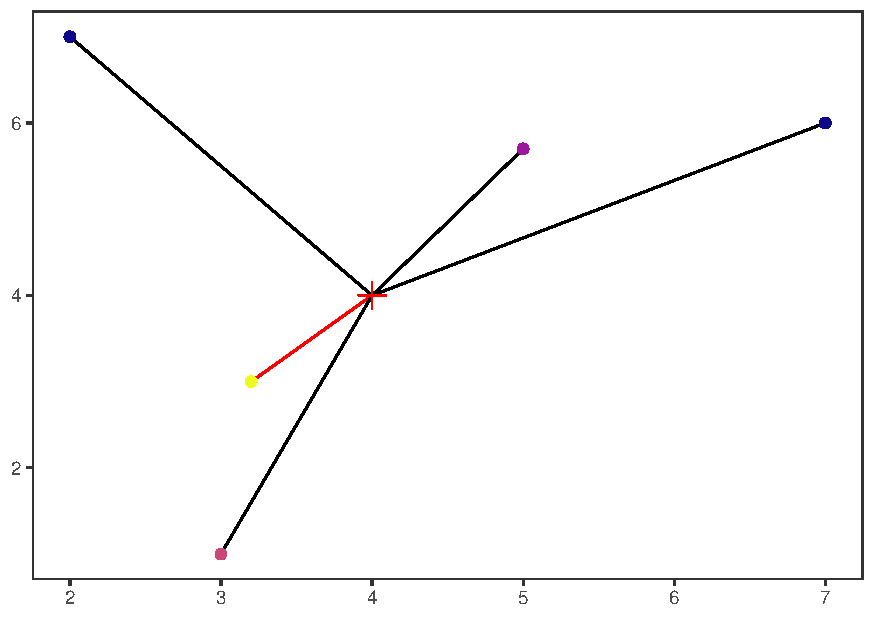
\includegraphics[width=\linewidth]{Images/nearest.pdf}
        \caption{Nearest Ground Monitoring Station}
        \label{fig:nearest}
    \end{subfigure}%
    \begin{subfigure}{.33\textwidth}
        \centering
        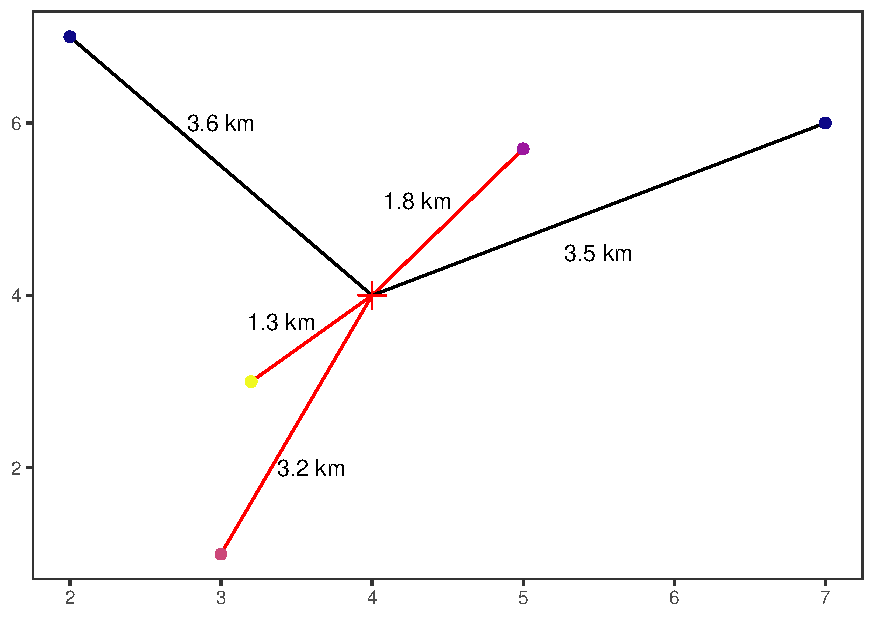
\includegraphics[width=\linewidth]{Images/inter.pdf}
        \caption{Distance Weighted Average of k-nearest Ground Monitoring Stations}
        \label{fig:inter}
    \end{subfigure}
    \begin{subfigure}{.33\textwidth}
        \centering
        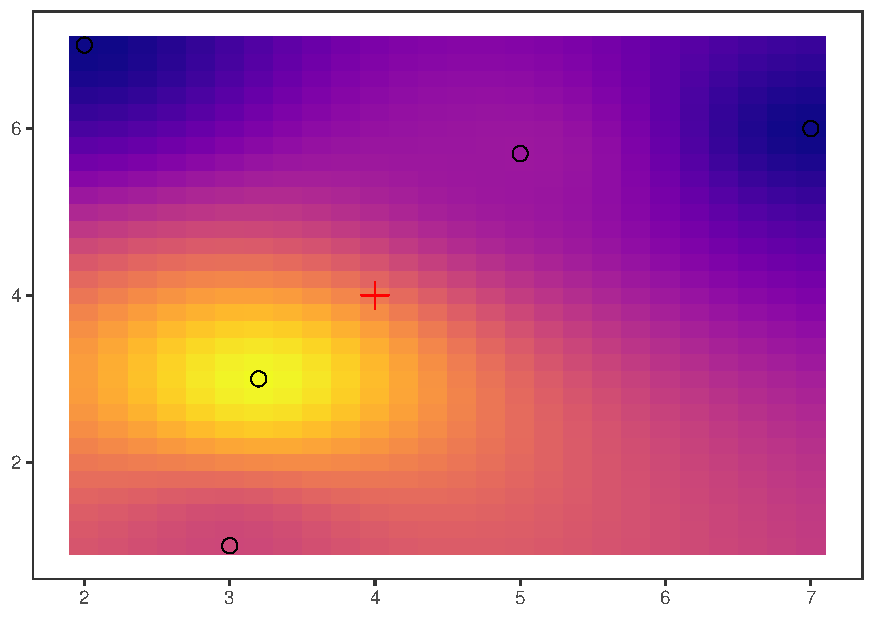
\includegraphics[width=\linewidth]{Images/interpol.pdf}
        \caption{Bilinear Interpolation of Ground Monitored Data}
        \label{fig:interpol}
    \end{subfigure}
\caption{Examples of Basic Methods for Using Ground Monitored Data for Individual Exposure Modelling}
\label{fig:monitormethods}
\end{figure}

Finally, interpolation methods of approximating air pollution concentrations underpin many spatial and spatial-temporal models, contrasting to the other methods, it allows estimation across an entire spatial domain for population-based studies, see Figure \ref{fig:interpol}. Many areas of literature explore the use of interpolation methods, both as the whole model and as part of a multistage or hierarchical model, with examples spanning across meteorological studies \citep{Haberlandt2007GeostatisticalEvent, Li2005SpatialPlateau}, exposure assessments \citep{Carnevale2021OptimalForecast}, and epidemiological risk measurements \citep{Congdon2013SpatiallyRisk, Blanco2018GeographicalTechnique}. The most basic approaches to interpolation are based on the Inverse Distance Weighted (IDW) algorithm, but also extend to triangulation methods, splines, geostatistical kriging, including Simple Kriging, Ordinary Kriging, and Bayesian Kriging, and, more recently, machine learning approaches, e.g. Random Forest (RF) \citep{Susanto2016SpatiotemporalModelling}. 

For interpolation of ground monitored air pollution data, a number of review articles have compared a subset of these approaches for particular pollutants and study domains. No one method has been shown to be both superior and computationally efficient for all cases and studies, hence the need for model selection and validation tools, such as through comparing error statistics, such as Root Mean Squared Error (RMSE) and Mean Absolute Error (MAE), and using cross-validation techniques.  

Most simply, the k-fold cross-validation method splits the data k times into a training and a testing set (of some specified size), then uses each training set to run the model and predict the cases in the test set to compare to the actual observed values in the testing set, see Figure \ref{fig:cross validation}. The case where the testing set is one less than the whole data set is called leave-one-out cross-validation (LOOCV), and is known as an extensive method but is however computationally expensive. \cite{Li2016SpatiotemporalApplication} using cross-validation to compare the use of different time scales for an interpolation method, whereas \cite{Lee2012ComparisonStates} uses cross-validation to compare the accuracy of two kriging based methods for ambient PM$_{2.5}$ in the US.

\begin{figure}
    \centering
    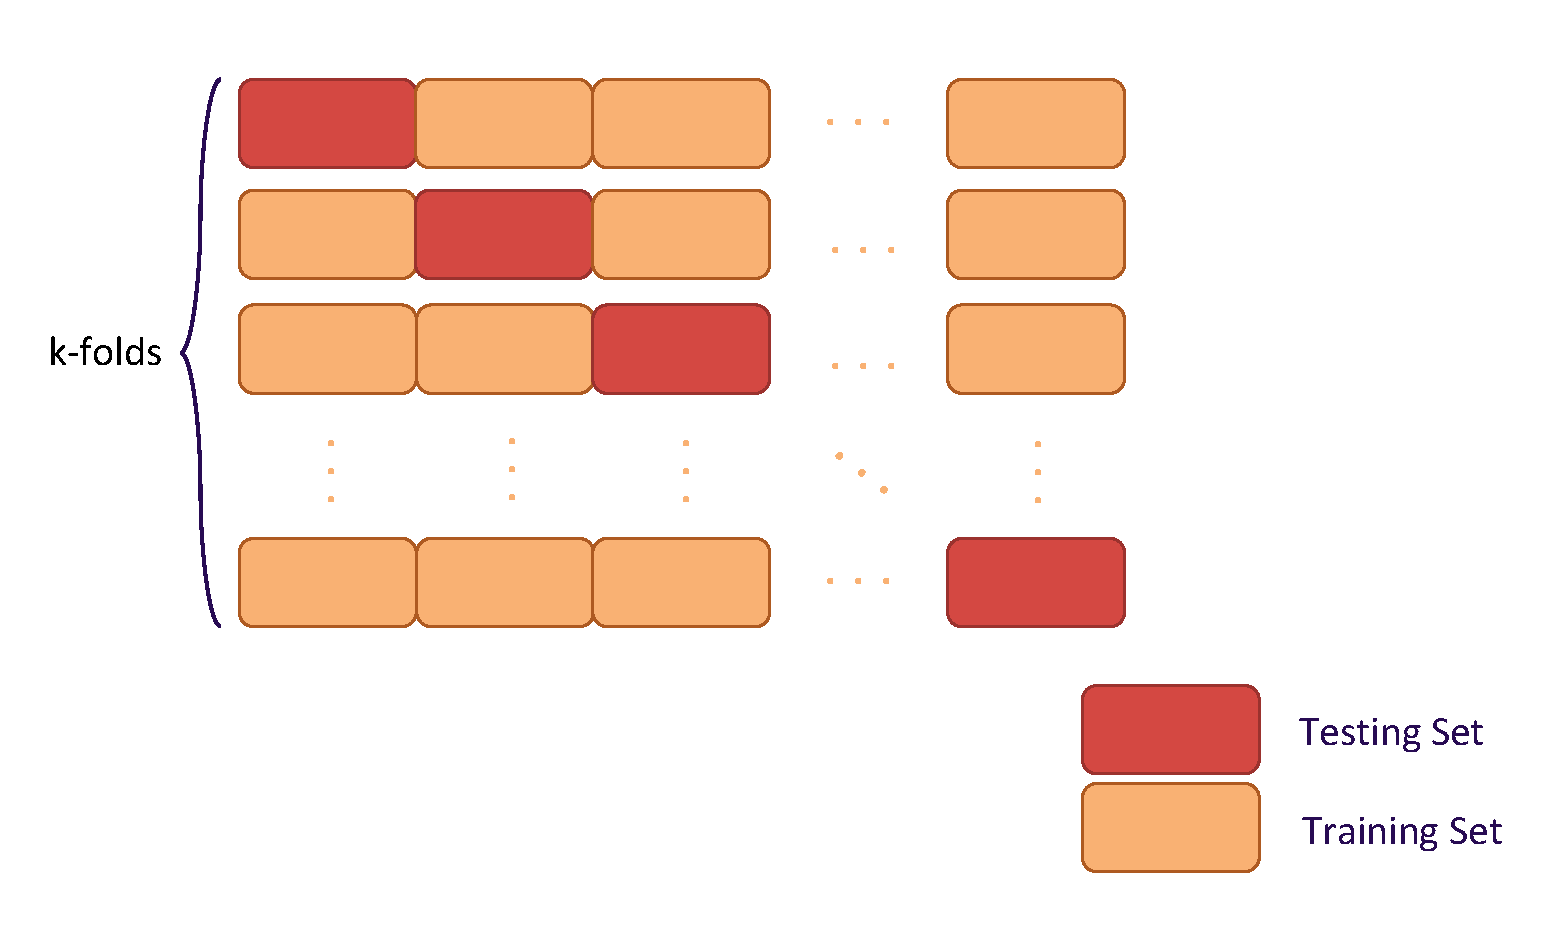
\includegraphics[width=0.7\linewidth]{Images/Cross-Validation.pdf}
\caption{Diagram of k-fold Cross-Validation}
\label{fig:cross validation}
\end{figure}

The main limitation to using purely ground monitored sources of air pollution data, is the current extent of global monitoring networks, these networks are usually expensive to set up and maintain, and, even in developed countries, lack evenly and thoroughly distributed sites. Out of the around 300 monitoring stations across the UK, there are 19 sites within the Greater London Urban Area (1,569 km\textsuperscript{2}) compared to only 6 in the Greater Manchester Area (1,276 km\textsuperscript{2}), and an even lower density in rural areas \textbf{ref map}. This discrepancy is further amplified between developed countries and low- and middle-income countries (LMIC), despite rising levels in air pollution and a higher burden of air pollution-based health impacts \citep{Bartington2020PrevalenceCountries}. Hence, the need for more sophisticated data collection and modelling approaches, for increased surveillance, evidence, and research of the global air pollution situation.

One key area of investigation to improve air quality monitoring in lower income countries, is the use of low-cost sensors, such as those discussed in \cite{Avis2020MonitoringCountries}, allowing for cheaper air pollution surveillance that can be used with traditional modelling approaches. However, as explored by a 2017 review by Hoek \citep{Hoek2017MethodsPollutants} a number of other approaches have provided significant improvements in this area, including: the use of satellite-derived data products \citep{Militino2018AnGeostatisticians, Zakeri2021AApplications, Zhang2021SatellitePerspectives}; land use classification and regression \citep{Knibbs2014AAustralia, VandenBossche2020ACarbon, Wang2020SpatiotemporalScale}; emissions and exposure data \citep{Saikawa2014GlobalN2Ob, Streets2013EmissionsCapability}; and Chemical Transport Models (CTMs) \citep{Beloconi2020BayesianModels, Chianese2018SpatiotemporallySimulations}. Other data sources such as meteorological variables and traditional numerical or physical models can also improve estimation and prediction in undermonitored areas, e.g. in \cite{Fasbender2009BayesianBelgium} and \cite{McMillan2010CombiningModelingd} respectively. 

However, the integration of multiple data sources imposes very large statistical, geographical, and computational problems. The main mathematical issue is the ‘change-of-support problem’ \citep{Gelfand2001OnData}, which addresses the exchangeablility of data between different units of spatial domain, primarily between point-referenced and areal data, but also between misaligned areal regions. Similarly, comparing and integrating sources of data using different spatial resolutions and units creates the so-called 'data misalignment' issue, \cite{Cameletti2019BayesianApproach} discusses the importance of addressing misalignment issues in exposure modelling and linkage to health data. The other major geographical consideration is the matching of coordinate reference systems (CRS), i.e. the map projection used to record and measure geographical distances on maps and globes. Also importantly, the computational burden of increasing the number of data sources may influence the selection of variables and modelling choices, especially when using large spatio-temporal datasets as discussed in \cite{Shekhar2015}. These modelling considerations underpin many challenges in this project, as the aim to create a complete and accurate exposure model for the UK will incorporate multiple sources of air pollution and meteorological data. 

\subsubsection{Satellite \textbf{Imagery? Approaches? Methods? Satellite-based Approaches}}
Recently satellite imagery has been growing rapidly in resolution, extent and accessibility. NASA remains the primary source of open access satellite imagery and hosts a range of instruments on various orbital paths over the Earth to measure different ranges of the electromagnetic spectrum at different spatial and temporal resolutions and extents \citep{NASA2021SVS:2021}. For air pollution measurements, the current key satellites are Aura, CALIPSO, OCO-2 and Sentinel-5P, which measure a range of different air pollution related values, both direct atmospheric concentrations, such as for Ozone and Nitrogen Dioxide (NO\textsubscript{2}) column measurements, and proxy measurements, such as aerosol optical depth (AOD) for particulate matter \citep{Gray2021MeetExpeditions}. 

what is AOD, how is it related to PM2.5
studies in other countries/across regions

uncertainty???

other studies using aod in UK/europe???

\subsubsection{Underlying Models}
avaliable for uk/europe
methods
use in other studies

 - Physical/Numerical Models e.g. PCM, the other one\\

\subsubsection{Meteorological Data} \label{Section:Met Data}
why the ones I chose???


%\subsubsection{Issues with Using Air Pollution Data}
   % -availability\\
   % -resolution and extent\\
   % -crs?? \\
   % -misalignment\\
   % -big data challenges\\
    
% Hence, the use of hybrid models for estimating air pollution concentrations has been proposed, incorporating both satellite and ground based measurements of air pollution to complete the picture \citep[e.g.][]{Kloog2014AData}.

%Another increasingly popular consideration in air pollution modelling and Public Health surveillance is land use. Land use is usually classified via satellite imagery and some ground knowledge of the area, and increasingly machine learning techniques are being used to accurately and efficiently classify different classes of land use and cover (\cite{NationalOceanicandAtmosphericAdministration2019}, \cite{Talukdar2020Land-UseReview}). With the two latest NASA Landsat missions, Landsat 8 and 9, there is now full Earth coverage every 8 days for visible and near infrared images \citep{Gray2021MeetExpeditions}, the most commonly used range in land use classification. Land use can play an important factor in local health outcomes, \citet{Dannenberg2003TheAgenda} presents a variety of considerations to how the built environment can affect our health and particularly focuses on the availability of greenspaces and the proximity to major roads, both of which are intrinsically linked to air pollution. Epidemiological studies involving land use have been used for a range of different health outcomes, such as pregnancy complications \citep[e.g.][]{Choe2018AirPregnancy} and common morbidities \citep[e.g.][]{Zock2018TheNeighbourhoods}. Along with more recent studies in the association between access to greenspaces and cognitive function and health; these include childhood behavioural outcomes \citep[e.g.][]{Madzia2019ResidentialOutcomes}, development of ADHD \citep[e.g.][]{Thygesen2020TheStudy}, bipolar disorder \citep[e.g.][]{Chang2021ResidentialTaiwan}, and adolescents’ cognition and mental health \citep[e.g.][]{Maes2021BenefitHealth}.

\subsection{Current Approaches}
Air pollution modelling and subsequent exposure models are predominately spatial or spatial-temporal statistics specialisms, with many of the modelling techniques and analysis based on the spatial spread and distribution of pollutants across a domain, and usually also over time. Due to this, many current approaches are based on or developed from core spatial statistics principals and models. Noel Cressie's book \textit{Statistics for Spatial Data} \citep{Cressie2015} is recognised within the field as a comprehensive guide to the fundamentals of spatial statistics, with the later \textit{Statistics for Spatio-temporal Data} \citep{Cressie2011StatisticsData} by Cressie and Wikle providing the extension to spatial-temporal statistical models. Spatial-temporal models naturally lend themselves to Bayesian modelling approaches, for the notions of conditional probabilities, prediction, hierarchical structures, and measures of uncertainty; Banerjee, Carlin and Gelfand extend these Bayesian Hierarchical modelling ideas for spatial and spatial-temporal data in their book \textit{Hierarchical Modelling and Analysis for Spatial Data} \citep{Banerjee2014}. These texts all explore the general set-up of using spatial data, in regards to definition of point-referenced and areal data, spatial scales and projections, and defining the basic three layers of a Bayesian Hierarchical Model (BHM): data model, process model, parameter model. 

Chapter 11 of \cite{Banerjee2014} discusses the general formulation of the most basic spatial-temporal BHM:
\begin{center}
$ Y(\textbf{s},t) = \mu(\textbf{s},t)  + e(\textbf{s},t), e(\textbf{s},t) \sim N(0, \Sigma)$ \\
$ \mu(\textbf{s},t) = \beta(\textbf{s},t) \textbf{X}(\textbf{s},t)$ \\
$ e(\textbf{s},t) = \omega(\textbf{s},t)  + \varepsilon(\textbf{s},t) $ \\
\end{center}
where $Y(\textbf{s},t)$ is the measurement at location \textbf{s} at time t, with mean structure $\mu(\textbf{s},t)$ and residuals $e(\textbf{s},t)$. $\textbf{X}(\textbf{s},t)$ are the covariates of measurement Y with coefficients $\beta(\textbf{s},t)$, $\omega(\textbf{s},t)$ are the spatial-temporal random effects to be defined, and the unstructured error is $\varepsilon(\textbf{s},t)$. Modelling considerations include the definition of the covariance function, $\Sigma = cov(Y(\textbf{s},t), Y(\textbf{s}',t')$, the form of the spatial-temporal random effects, e.g. $\omega(\textbf{s},t) = \alpha(t) + \omega(\textbf{s})$, and the dependence of the coefficients, i.e. $\beta = \beta, \beta(\textbf{s}), \beta(t), \beta(\textbf{s},t)$.

More specifically to the field of exposure assessment \textit{Handbook of Environmental and Ecological Statistics} \citep{Gelfand2019HandbookStatistics} outlines many of the previously discussed interpolation methods (including kNN, IDW, and Bayesian Kriging) and two key data fusion methods (downscaling and Bayesian melding), with an application to PM$_{2.5}$. Alternative popular approaches in the Bayesian spatial-temporal modelling of air pollution include Bayesian inversion, coming from the modelling of trajectories of air pollutants over space and time \citep{Bergamaschi2000InverseRatios}, and Bayesian Maximum Entropy, which uses a similar approach to BHM to integrate hard and soft data sources \citep{He2018BayesianReview}.

This project is designed to present a new approach to air pollution modelling and assessment in the UK, utilising a Bayesian framework, spatiotemporal modelling methods, and the integration of multiple sources of air pollution data. To be modern, up-to-date, and novel, an investigation into the current methodologies in this area will provide a solid starting point for methods development and modelling strategies. Following the recommendations by \cite{Grant2009AMethodologies}, a mixed methods review presents a structured and vigorous way to identify and evaluate such existing literature and methodologies \textbf{in global publications}.

\subsubsection{Search Strategy}
A comprehensive search of publications was completed by including 4 major publication databases related to the fields of environmental science, mathematics and epidemiology: Scopus, Web of Science, PubMed, and GeoRef. The definitive search was conducted on the 15th June 2022 and was open to all publication dates available on the search sites. 

4 main category words for the search were identified: air pollution, Bayesian, multisource, and spatiotemporal, with the subsequent search terms stemming from these \ref{table:Search terms}. The final search combined these categories with an ADD operator to ensure all requirements were met.

\begin{table}[h!]
\centering
\begin{tabular}{c p{11cm}} 
 Category & Search Terms \\ [0.5ex] 
 \hline
  Air Pollution & "air pollution" OR "air quality" OR "air pollut*" OR "particulate matter" OR "particulates" OR "nitrogen dioxide" OR "NO2" OR "sulphur dioxide" OR "SO2" OR "ozone" OR "O3" OR "volatile organic compounds" OR "vocs" OR "air index" OR "pollutant" \\ 
  Bayesian & "bayesian" OR "bayes*" \\
  Multisource & "multisource" OR "multi-source" OR "multiple sources" OR "data integrat*" OR "source integrat*" OR "many sources" OR "sources" \\ 
  Spatiotemporal & "spatiotemporal" OR "spatio-temporal" OR "spatial temporal" OR "space-time" OR "space time" OR "spatialtemporal" OR "spatial-temporal" OR "time space" \\ [0.5ex]
 \hline
\end{tabular}
\caption{Search Term used in Systematic Search for Methods}
\label{table:Search terms}
\end{table}

As per the methods review methodology as defined by \cite{Grant2009AMethodologies}, the primary research questions of this review are:

\begin{enumerate}
    \item How many publications have approached air pollution modelling through a multisource Bayesian spatiotemporal lens? Are there any regional or temporal trends in these?
    \item Which Bayesian methodologies have been considered and are currently used? 
    \item Which air pollutants are more commonly investigated? 
    \item Which sources of air pollution data and models are being used? Particularly for the UK and Europe.
\end{enumerate}

\subsubsection{Screening Procedure}
Following the identification of 660 publications (including journal articles, book chapters, and conference proceedings), the initial screening process, completed using the Mendeley Reference Management Software, removed all duplicated entries, prioritising Scopus as the main source of article information and content.

\subsubsection{Inclusion Eligibility} 
Inclusion eligibility was considered in three stages: a title review, an abstract review, and a full-text review. Primary reasons for exclusion involved the study not being directly related to air pollution and studies that did not specifically use multiple sources of air pollution data, including ground monitoring data, satellite data, and physical/numerical modelling data.

\tikzstyle{start} = [rectangle, minimum width=3cm, minimum height=1cm, text centered, text width = 9cm, draw=black, fill=none]
\tikzstyle{left} = [rectangle, minimum width=3cm, minimum height=1cm, text centered, text width = 5cm, draw=black, fill=none]
\tikzstyle{right} = [rectangle, minimum width=3cm, minimum height=1cm, text centered, text width = 9cm, draw=black, fill=none]
\tikzstyle{arrow} = [thick,->,>=stealth]



\begin{figure}
    \centering
    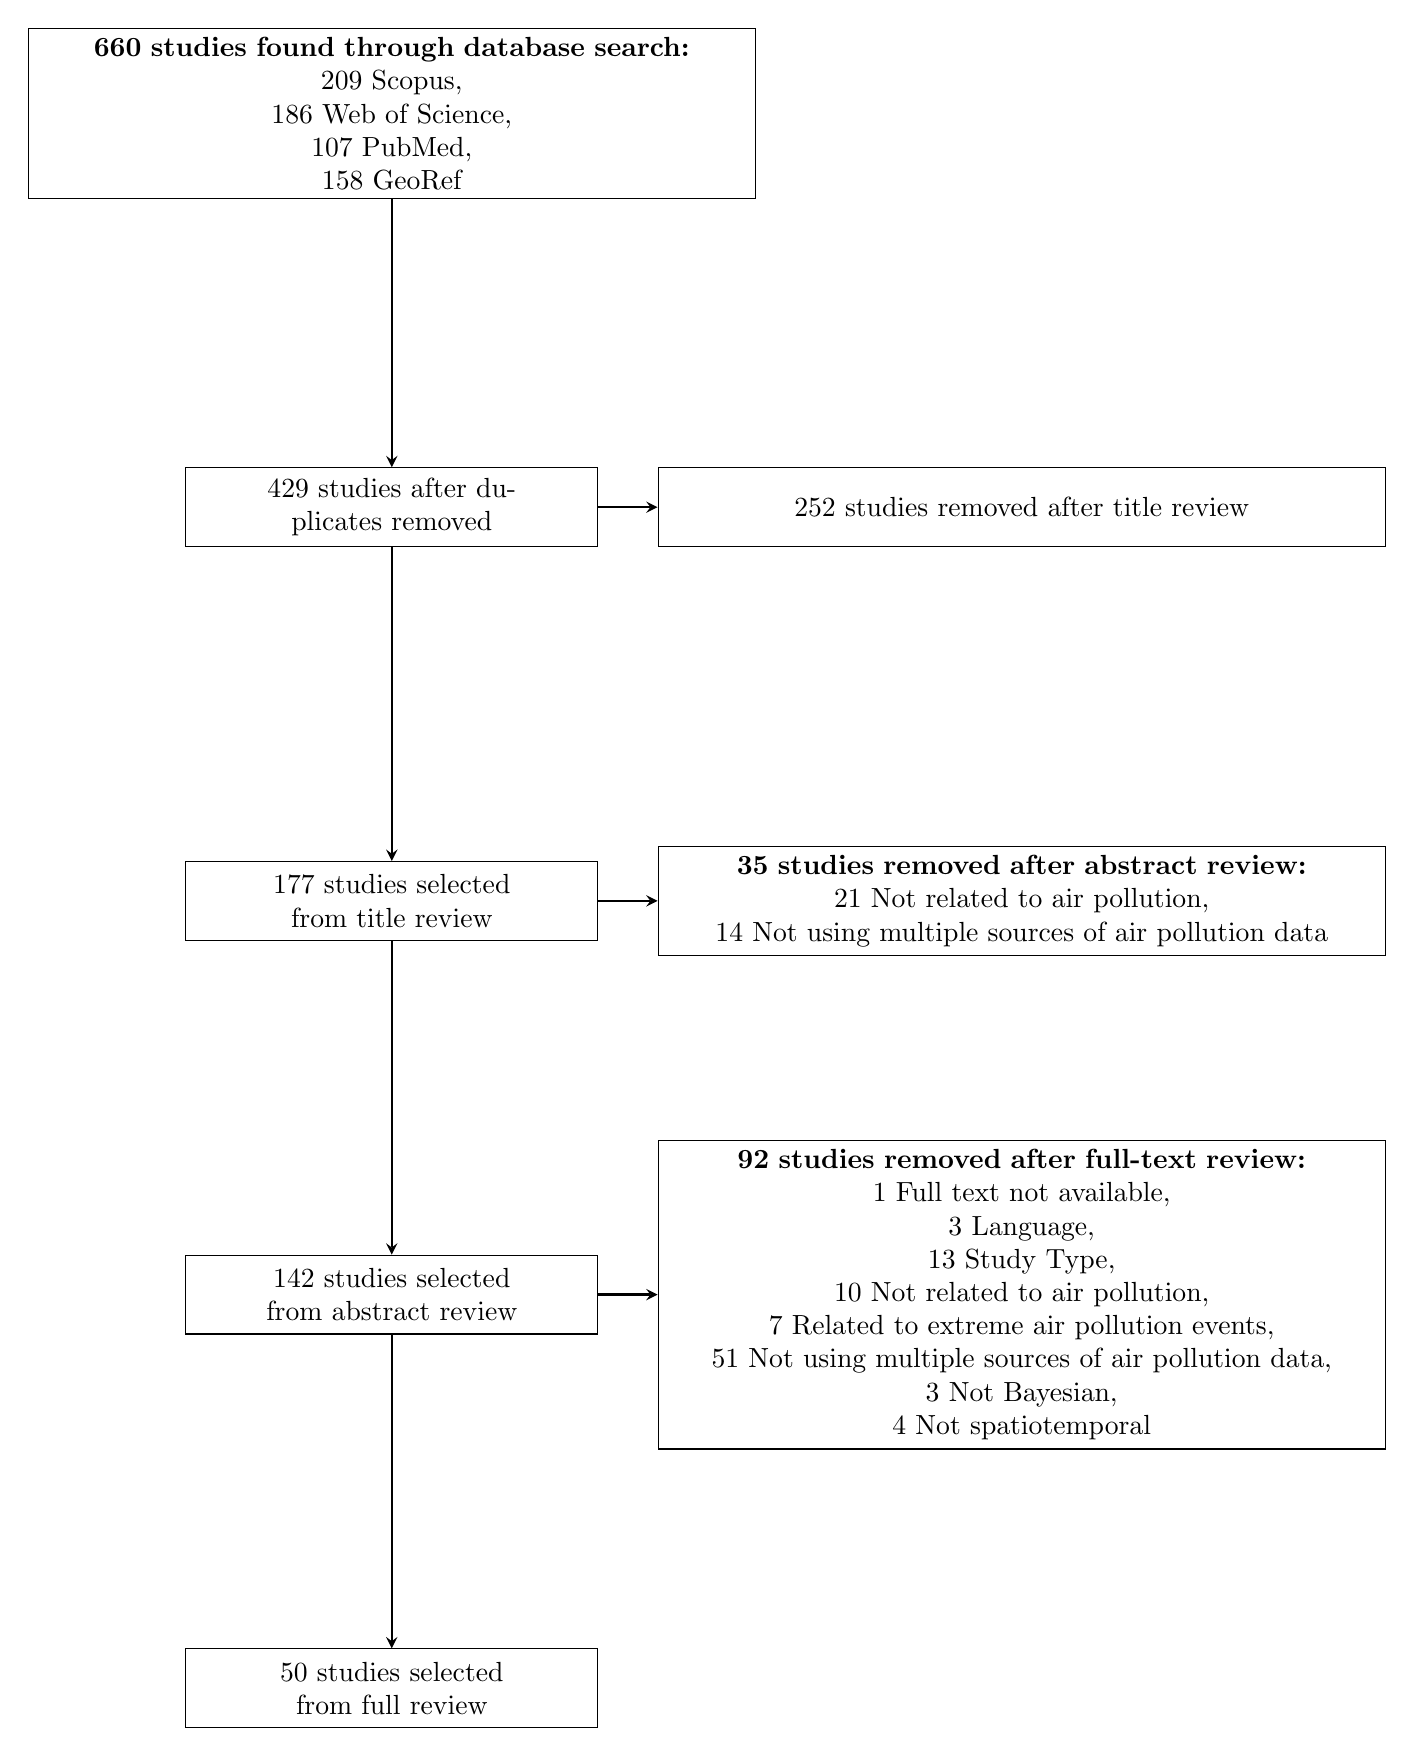
\begin{tikzpicture}[node distance=8cm]
        \node (All Results) [start] {\textbf{660 studies found through database search:} \\ 209 Scopus,\\ 186 Web of Science,\\ 107 PubMed,\\ 158 GeoRef};
        \node (Duplicates) [left, below of = All Results, yshift = 3cm] {429 studies after duplicates removed};
        \node (Title Exclude) [right, right of = Duplicates] {252 studies removed after title review};
        \node (Title Include) [left, below of = Duplicates, yshift = 3cm] {177 studies selected from title review};
        \node (Abstract Exclude) [right, right of = Title Include] {\textbf{35 studies removed after abstract review:} \\ 21 Not related to air pollution, \\ 14 Not using multiple sources of air pollution data};
        \node (Abstract Include) [left, below of = Title Include, yshift = 3cm] {142 studies selected from abstract review};
        \node (Full Text Exclude) [right, right of = Abstract Include] {\textbf{92 studies removed after full-text review:} \\ 1 Full text not available, \\ 3 Language, \\ 13 Study Type, \\ 10 Not related to air pollution, \\ 7 Related to extreme air pollution events, \\ 51 Not using multiple sources of air pollution data, \\ 3 Not Bayesian, \\ 4 Not spatiotemporal };
        \node (Full Text Include) [left, below of = Abstract Include, yshift = 3cm] {50 studies selected from full review};

        \draw [arrow] (All Results) -- (Duplicates);
        \draw [arrow] (Duplicates) -- (Title Exclude);
        \draw [arrow] (Duplicates) -- (Title Include);
        \draw [arrow] (Title Include) -- (Abstract Exclude);
        \draw [arrow] (Title Include) -- (Abstract Include);
        \draw [arrow] (Abstract Include) -- (Full Text Exclude);
        \draw [arrow] (Abstract Include) -- (Full Text Include);
    \end{tikzpicture}
\caption{PRISMA-Based Flow Diagram for the systematic literature search of methods}
\label{fig:methods review}
\end{figure}

\subsubsection{Results}
The mixed methods review initially identified 429 unique publications and resulted in 52 finally included studies (see Table \ref{fig:methods review}). 

\begin{landscape}
\begin{longtable}{c p{4cm} c p{4cm} p{6cm}}
\textbf{Main Modelling Approach} & \textbf{Source} & \textbf{Region} & \textbf{Air Pollutants} & \textbf{Air Pollution Data Sources} \\

 Bayesian Data Fusion & \cite{Fasbender2009BayesianBelgium} & Belgian & NO\textsubscript{2} & Ground, Emission Data  \\

 Bayesian Ensemble Machine Learning & \cite{Ren2022FlexibleConcentrations} & US & O\textsubscript{3} & Ground, CMAQ Model, Land Use \\

 Bayesian Hierarchical Model & \cite{Beloconi2020BayesianModels} & Europe & NO\textsubscript{2} & Ground, GEOS-Chem and CAMs Models, Satellite  \\
 
 & \cite{Berrocal2010AMisalignment} & US & O\textsubscript{3} & Ground, CMAQ Model  \\

 & \cite{Blangiardo2016Two-stagePrescriptions} & UK & NO\textsubscript{2} & Ground, AMDS-Urban Model  \\

 & \cite{Boaz2019MultivariateMissingness} & US & CO, EC, NH\textsubscript{4}, NO\textsubscript{2}, O\textsubscript{3}, PM\textsubscript{2.5}, SO\textsubscript{2}, SO\textsubscript{4} & Ground, CMAQ Model  \\

  & \cite{Braggio2022NewHospitalizationsb} & US & PM\textsubscript{2.5} & Ground, CMAQ Model \\

 & \cite{Choi2009MultivariateParticles} & US & PM\textsubscript{2.5} & Ground, CMAQ Model  \\

  & \cite{Crooks2013AFieldb} & US & CO, NO\textsubscript{x}, PM\textsubscript{2.5}  & Ground, CMAQ and AERMOD Models  \\

  & \cite{Fioravanti2021Spatio-temporalApproachb} & Italy & PM\textsubscript{10} & Ground, Satellite  \\
  
  & \cite{Forlani2020AR-INLAd} & UK & NO\textsubscript{2} & Ground, AQUM and PCM Models \\
 
  & \cite{Gilani2019NonstationaryEnvironmentb} & US & NO\textsubscript{x}, PM\textsubscript{2.5} & Ground, RLINE Model  \\
  
  & \cite{Huang2015AnScotlandb} & UK & NO\textsubscript{2} & Ground, PCM Model  \\
  
 & \cite{Huang2018MultivariateUncertaintyb} & UK & NO\textsubscript{2}, PM\textsubscript{10} & Ground, PCM Model  \\ 
 
 & \cite{Lee2017AHealthb} & UK & NO\textsubscript{2}, O\textsubscript{3}, PM\textsubscript{2.5}, PM\textsubscript{10} & Ground, AQUM Model  \\
 
  & \cite{Liang2013Time-spaceDatasets} & US & PM\textsubscript{2.5} & Ground, Satellite  \\
  
 & \cite{Lv2017DailyObservations} & China & PM\textsubscript{2.5} & Ground, Satellite  \\
 
  & \cite{McMillan2010CombiningModelingd} & US & PM\textsubscript{2.5} & Ground, CMAQ Model  \\
  
  & \cite{Mukhopadhyay2018AWalesb} & UK & NO\textsubscript{2}, O\textsubscript{3}, PM\textsubscript{2.5}, PM\textsubscript{10} & Ground, AQUM Model  \\
  
 & \cite{Murray2019ASimulationb} & US & PM\textsubscript{2.5} & Ground, CMAQ Model, Satellite  \\
 
  & \cite{Paciorek2012AssessmentStates.} & PM\textsubscript{2.5} & Ground, CMAQ Model, Satellite  \\
  
  & \cite{Pirani2014BayesianAreas} & UK & PM\textsubscript{10} & Ground, AMDS-Urban Model  \\
  
   & \cite{Sahu2009ImprovedUSb} & US & O\textsubscript{3} & Ground, CMAQ Model  \\
   
 & \cite{Sahu2012HierarchicalData} & US & O\textsubscript{3} & Ground, CMAQ Model  \\
  
  & \cite{Sahu2015BayesianStates} & US & O\textsubscript{3} & Ground, CMAQ Model  \\
 
   & \cite{Sun2021Multi-stageModelsb} & World & O\textsubscript{3} & Ground, CMPI6 Model  \\
   
  & \cite{Turner2016Long-TermStudy} & US & O\textsubscript{3} & Ground, CMAQ Model \\
  
 Bayesian Inversion & \cite{Bergamaschi2000InverseRatios} & World & CO & Ground, TM2 Model  \\
 
   & \cite{Breon2015AnMeasurements} & France & CO\textsubscript{2} & Ground, CHIMERE Model  \\
   
  & \cite{Chianese2018SpatiotemporallySimulationsc} & Italy & PM & Ground, CAMS Model \\
  
 & \cite{Cui2019A2014-2016} & US & CH\textsubscript{4} & FLEXPART-WRF Model, Aircraft and Tower Data   \\
 
  & \cite{Cui2019InversionMeasurements} & US & CH\textsubscript{4} & FLEXPART-WRF Model, Aircraft Data, Emissions Data \\
  
   & \cite{DeFoy2015EstimatingSupersite} & US & EC, OC & Ground, CAMx Model  \\
   
   
  & \cite{Heald2004ComparativeMonoxide} & Asia & CO & Satellite, Aircraft Data  \\
  
 & \cite{Jia2021BlackChina} & China & BC & Ground, Emissions Data  \\
  
   & \cite{Lopez-Coto2020WintertimeTechnique} & US & CH\textsubscript{4}, CO, CO\textsubscript{2} & Ground, Ensemble of Models, Emissions Data  \\
   
  & \cite{Saikawa2014GlobalN2O} & World & N\textsubscript{2}O & Ground, MOZART Model  \\
  
 & \cite{Souri2016ConstrainingCampaign} & US & NO\textsubscript{2}, NO\textsubscript{x} & Ground, CMAQ Model, Satellite  \\
 
   & \cite{Stavrakou2006Grid-basedDatab} & World & CO & IMAGES and MOPITT Models, Emissions Data  \\
   
  & \cite{Turner2016Long-TermStudy} & US & CO\textsubscript{2} & Ground, STILT Model  \\
  
 Bayesian Maximum Entropy &  \cite{deNazelle2006OzonePrediction} & US & O\textsubscript{3} & Ground, MAQSIP Model  \\
   
   & \cite{Delang2021Mapping1990-2017b} & World & O\textsubscript{3} & Ground, Ensemble of Models  \\
   
  & \cite{He2018Space-timeApproachc} & China & PM\textsubscript{2.5} & Ground, Satellite  \\

  & \cite{He2020Space-timeTechniques} & China & PM\textsubscript{2.5} & Ground, MERRA Model, Satellite  \\
  
 & \cite{Xiao2018High-resolutionTechnique} & China & PM\textsubscript{2.5} & Ground, Satellite  \\
 
  & \cite{Xu2016BayesianApplicationb} & US & O\textsubscript{3} & Ground, CAMx Model  \\
  
   & \cite{Xu2017ImpactMisclassificationb} & US & O\textsubscript{3} & Ground, CAMx Model  \\
   
 Bayesian Markov Random Fields & \cite{Gong2021MultivariateINLA.} & US & CO, EC, NH\textsubscript{4}\textsuperscript{+}, NO\textsubscript{2}, NO\textsubscript{3}\textsuperscript{-}, NO\textsubscript{x}, O\textsubscript{3}, OC, PM\textsubscript{2.5}, PM\textsubscript{10}, SO\textsubscript{2}, SO\textsubscript{4}\textsuperscript{-} & Ground, CMAQ Model  \\
  
 & \cite{Western2020BayesianFieldsc} & UK & CH\textsubscript{4} & Ground, NAME III Model  \\
 
 Bayesian Neural Network & \cite{Sun2021Multi-stageModelsb} & World & O\textsubscript{3} & Ground, CMIP6 Model \\
 
\caption{Studies and Methods Identified in the Methods Review}
\label{table:Methods Review}
\end{longtable}
\end{landscape}

\begin{figure}
    \centering
    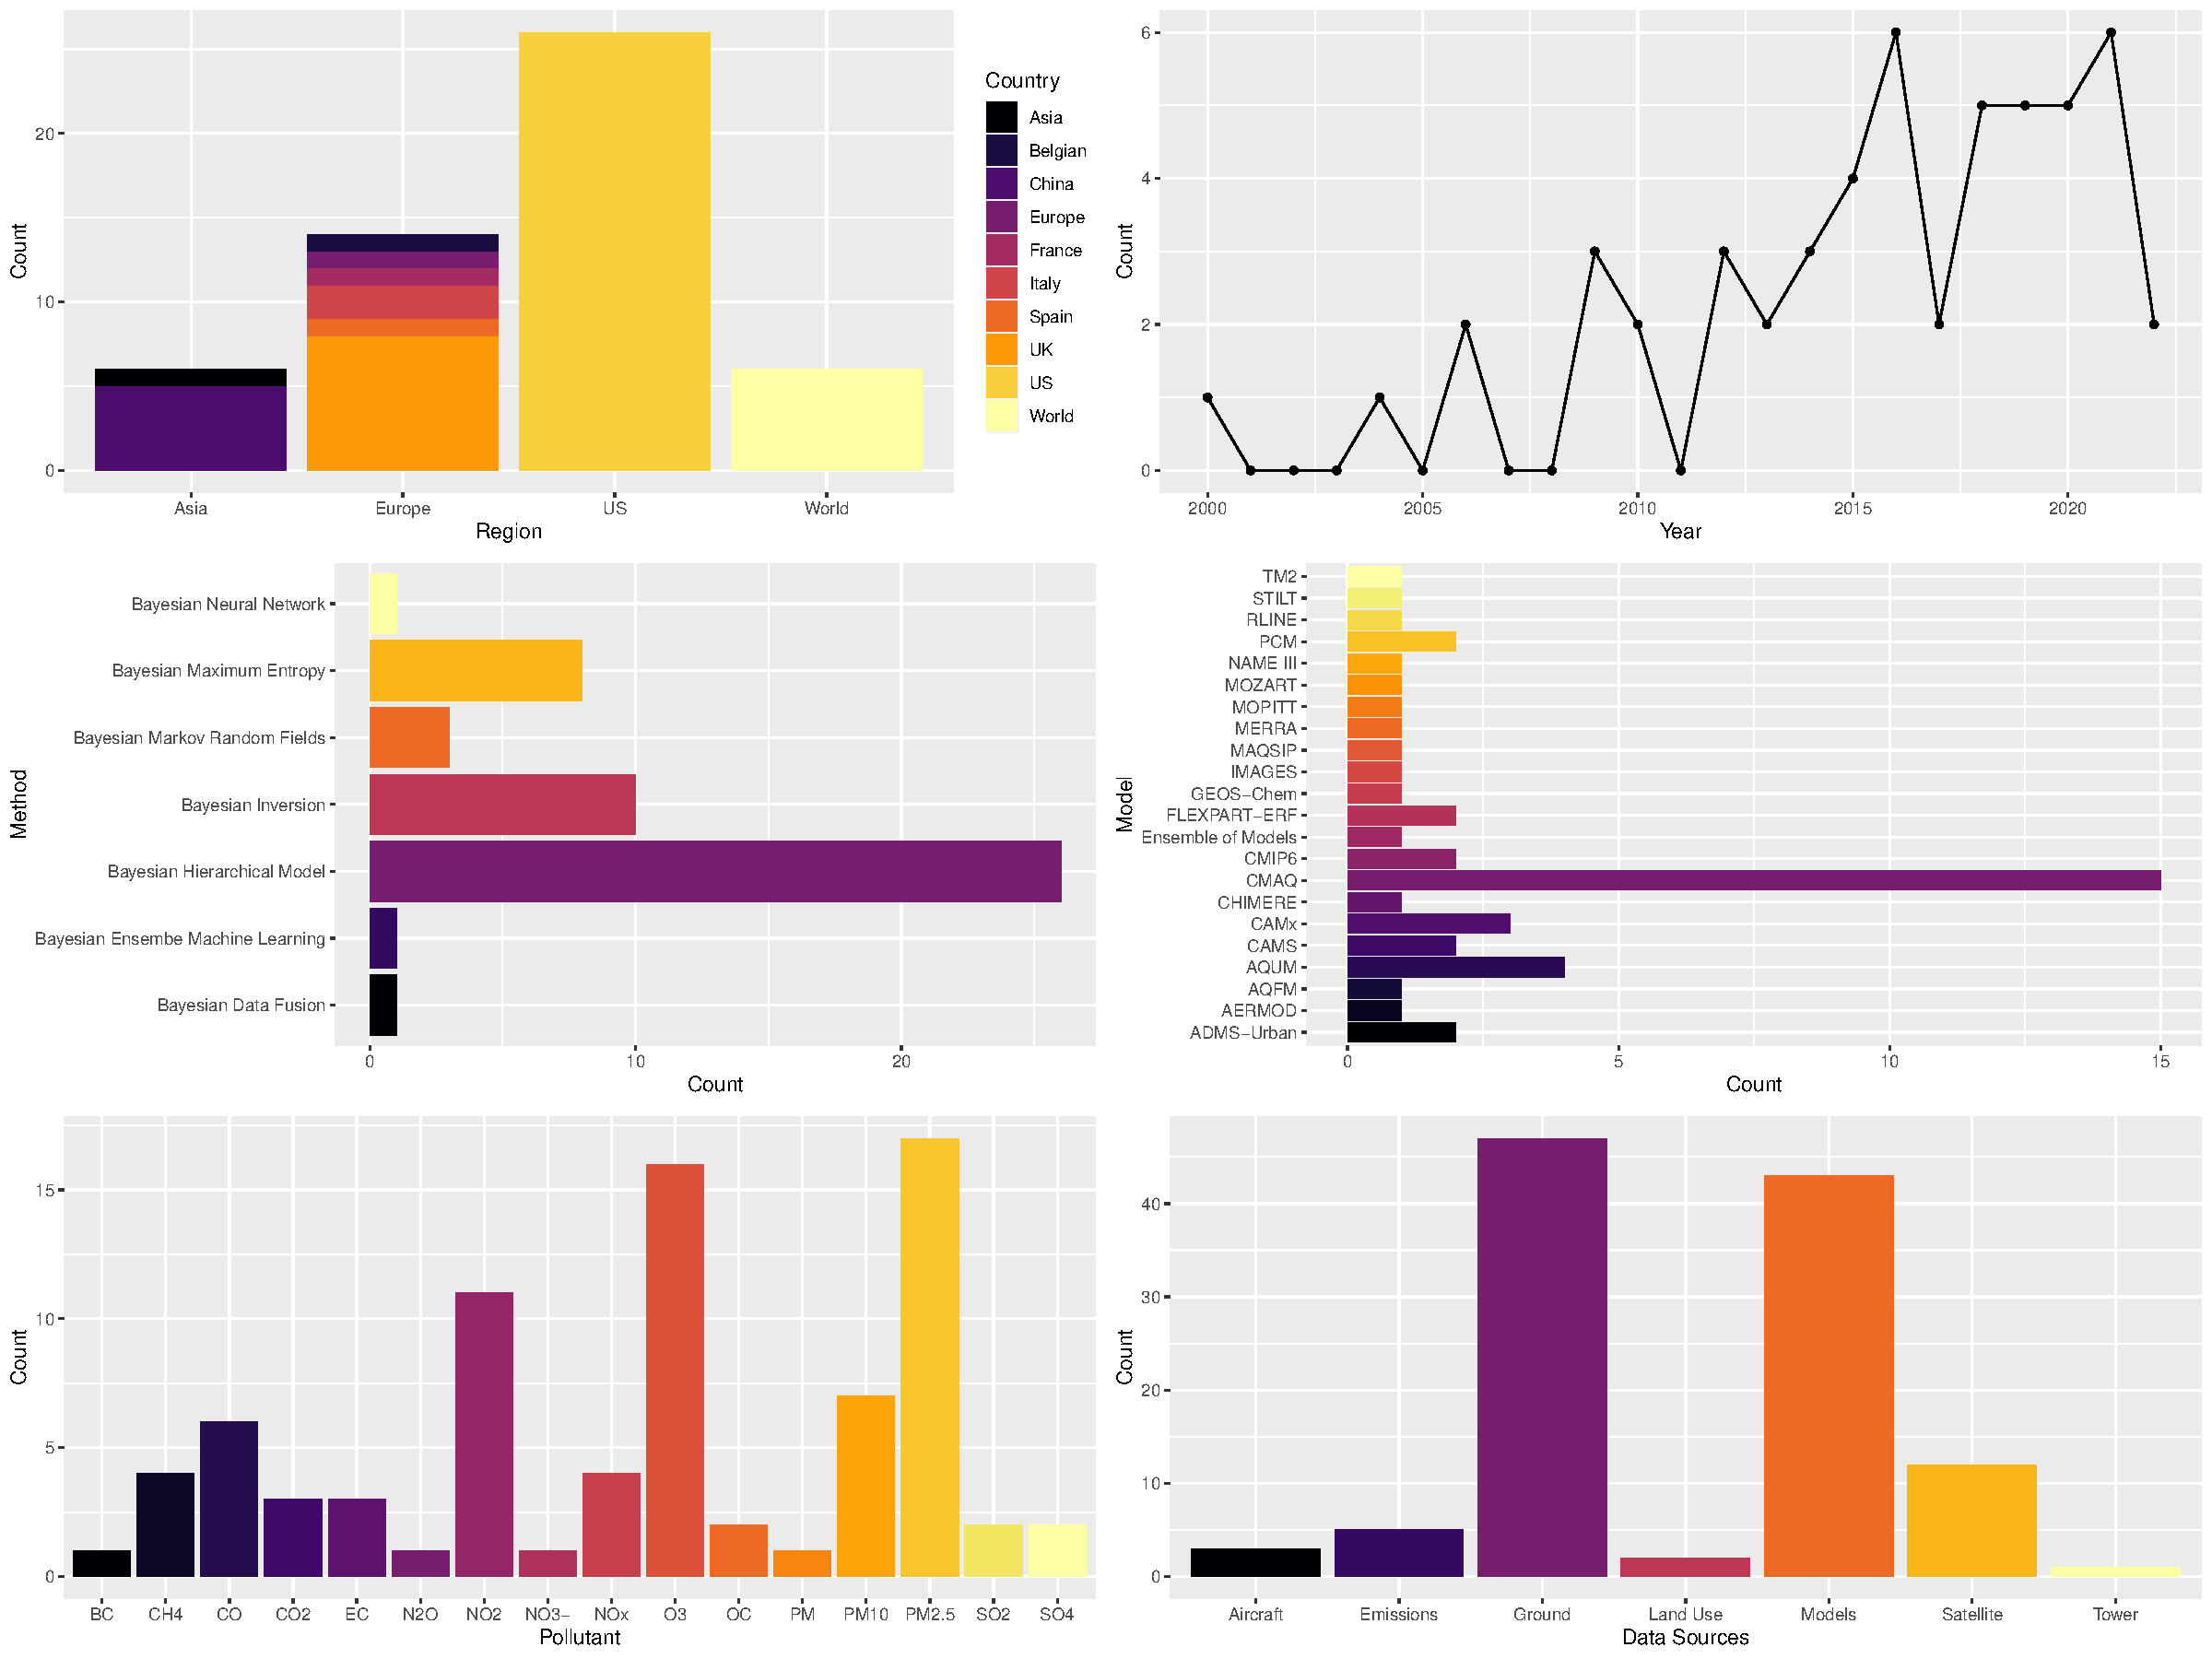
\includegraphics[width=\linewidth]{Images/Methods Review.pdf}
\caption{Results of the Methods Review}
\label{fig:methodsreview}
\end{figure}

\subsubsection{Discussion}
\textbf{Research Question 1} \\
Of the 52 studies identified through this methods review, we see a number of different trends in region of interest and publication dates. Half of studies (26) using these methods consider the US or areas within the US, then many others consider areas in Europe (14) and Asia (6), with 8 studies focusing on the UK. Furthermore, 6 studies extend their interests to the entire world, usually working at larger spatial resolutions. Interestingly, there are no studies that specifically look at the African, South American, nor Australia/Oceania continents. 

The other predominant trend in these publications is the general increase over time, the first study identified through this review is from 2000 and over 20 from the last 5 years alone. Although these numbers remain relatively low (only 6 studies in 2021), it does seem to be an area of research that is gaining interest and traction in the recent years.

\textbf{Research Question 2}\\
Identifying the methods used in these studies was an interesting process, methods such as Bayesian Neural Networks, Bayesian Maximum Entropy and Bayesian Inversion were easy to recognise, the language was consistent across publications and research areas. Whereas differentiating between more general modelling approaches was more difficult. Bayesian Hierarchical Modelling (BHM) is a broad framework into which more specific modelling strategies and specifications can be made, for example, many of the studies classified as Bayesian Hierarchical Modelling use methods such as Bayesian Melding and Downscaling as data fusion approaches, however some studies may have used these approaches but do not name or specify them as such. Also within this category, studies may use methods of kriging, land use regression, non-stationary models, and latent fields, but due to the language used and lack of specificity they have been consider under the umbrella of BHM. Due to this, BHM was the largest identified category of method, followed by Bayesian Maximum Entropy and Bayesian Inversion. 

Bayesian Maximum Entropy (BME) is most generally a framework in which to integrate multiple data sources in a spatial or spatiotemporal model, most commonly categorised into soft and hard data. The theory of BME is presented and reviewed in \cite{He2017BayesianReview}, it has shown great predictive accuracy compared to some kriging approaches, with the most common applications in environmental and social sciences. Bayesian Inversion is a more specific computational method used for approximating modelling inputs from the outputs, more specifically in air pollution modelling, it aims to approximate trajectories of air pollutants through dispersion, chemical transport, and emissions models, such as using the FLEXPART-WRF model in \cite{Cui2019InversionMeasurements}.

\textbf{Research Question 3}\\
Parallel to background research and the wider field of air pollution modelling, the primary pollutants of interest in these studies are Particulate Matter 2.5 (PM$_2.5$), Ozone (O$_3$), and Nitrogen Dioxide (NO$_2$). 

\textbf{Research Question 4}\\
As for the air pollution data sources used, ground monitored data was used across all but 3 of the studies, primarily coming from national monitoring networks. Following this, underlying models were the next most common source of air pollution data (43 studies), with many different types and sources of model being used. The Community Multiscale Air Quality (CMAQ) model was the primary model of choice over all the studies, it is a multi-faceted model for the US integrating an air-chemistry transport model with both emissions and meteorological models. Whereas, for the UK, there was not one clear outlying model that was common across multiple studies. For the European model in \cite{Beloconi2020BayesianModels}, the Goddard Earth Observing System Chemical Transport (GEOS-Chem) model and the Copernicus atmosphere monitoring service (CAMS) model were used, taking advantage of the chemical transport simulations and meterological variables in the GEOS-Chem, and the reanalysed ensemble of numerical models in the CAMS model: which integrates 8 regional numerical models across Europe. Then specifically for the UK, 4 models were included in different studies: ADMS-Urban, AQUM, NAMES III, PCM. With the Met Office's Air Quality in the Unified Model (AQUM) being the most used (4 studies). Each of these physical or numerical models have taken a slightly different approach: the ADMS-Urban model is a local urban city model integrating activity data, such as traffic, and buildings into the model; AQUM uses simulated aerosol chemical transports and emissions at a high temporal resolution; NAMES III is a Lagrangian air pollution dispersion model; and Defra's PCM model is a collection of models for each pollution, provided at a high spatial resolution for the UK.

The lack of the use of satellite data within these multisource models is also interesting, with only 12 studies including it in their models and none of the UK studies utilising it. This is surprising with the rising literature and evidence supporting the use of satellite-based air quality measurements for air pollution surveillance, as a complement or alternative to dense ground monitoring networks.

\subsubsection{Conclusion}
On review of the currently literature in this area, a number of conclusions can be made, especially on the research gaps and emerging methodologies. It is evident that the UK is not a primary location of interest, and many of the UK-based studies are regional based, e.g. Scotland or Greater London, or concentrate on NO$_{2}$ as the main pollutant; leaving a high-spatial resolution national PM$_{2.5}$ model fairly under-developed. Similarly, it is of particular novel interest to incorporate satellite-derived air pollution measurements into such a Bayesian multisource model, fulfilling a wide research gap that has been successful elsewhere.

\subsection{Significance and Application of the Approach}
The primary significance of this modelling approach is the incorporation of many modern techniques and frameworks, but also the expected spatial resolution and scale of the exposure model provides another layer of complexity. Bayesian statistical methods underpin many recent advances in data analysis and modelling \citep{vandeSchoot2021BayesianModelling}, and there is increasing global interest in applying these methods across disciplines and applications, especially areas with increasingly large data considerations, such as environmental and health modelling. Modern Bayesian hierarchical modelling and data integration methods allow for more sources of data to be considered, in this case utilised through the relatively novel use of integrating ground monitoring data, satellite data, underlying models, and meteorological variables. Additionally, the improvements in processing power, new R packages, and useful approximation methods give rise to more flexible, complex and larger spatial-temporal models, see the discussion of using R-INLA in \cite{Bakka2018SpatialReview}.

Also importantly, many modelling choices are selected to be concordant with the expected health datasets to be used in Objective 2 of the PhD project, for example the spatial extent covers the study areas of both the Biobank database and the SCAMP cohort, and the 1km x 1km spatial resolution matches the home residences given by the Biobank (See Section \ref{Health Methods}).



\section{Research Methods}
\label{ch:methods}

\subsection{Study Domain}
The spatial domain of the region of interest covers the island of Great Britain, including England, Scotland and Wales. This area was chosen to match the spatial domain of the Pollution Climate Mapping (PCM) model, described below, excluding Northern Ireland, and the extent of the residential addresses of the UK Biobank, again described below. For consistency, the study domain is projected to the 1km x 1km British National Grid (BNG) using Eastings and Northings in meters as units. 

For clipping and mapping of the full domain, the Office for National Statistics (ONS) full resolution digital vector boundary shapefiles for Great Britain, as of 31st December 2017, are used. As for the preliminary London studies, the Greater London Authority (GLA) statistical GIS boundary shapefiles for Greater London, as of 3rd May 2018, are chosen.

\subsection{Data}
\subsubsection{Ground Monitoring Data} 
The Automatic Urban and Rural Network (AURN) is the UK's largest automatic monitoring network and is used widely air quality reporting and research. With 172 current monitoring sites and 275 sites in total since 1972, it measures a range of pollutants, including coarse and fine particulate matter (PM$_{10}$, PM$_{2.5}$), Nitrogen Dioxide (NO$_{2}$), Ozone (O$_{3}$), and Sulphur Dioxide (SO$_{2}$). Predominately, the measurements are taken hourly, but for this application the monthly means are taken from the published summary statistics supplied by Defra. \ref{fig:aurn} shows ... 

\begin{figure}[h]
    \centering
    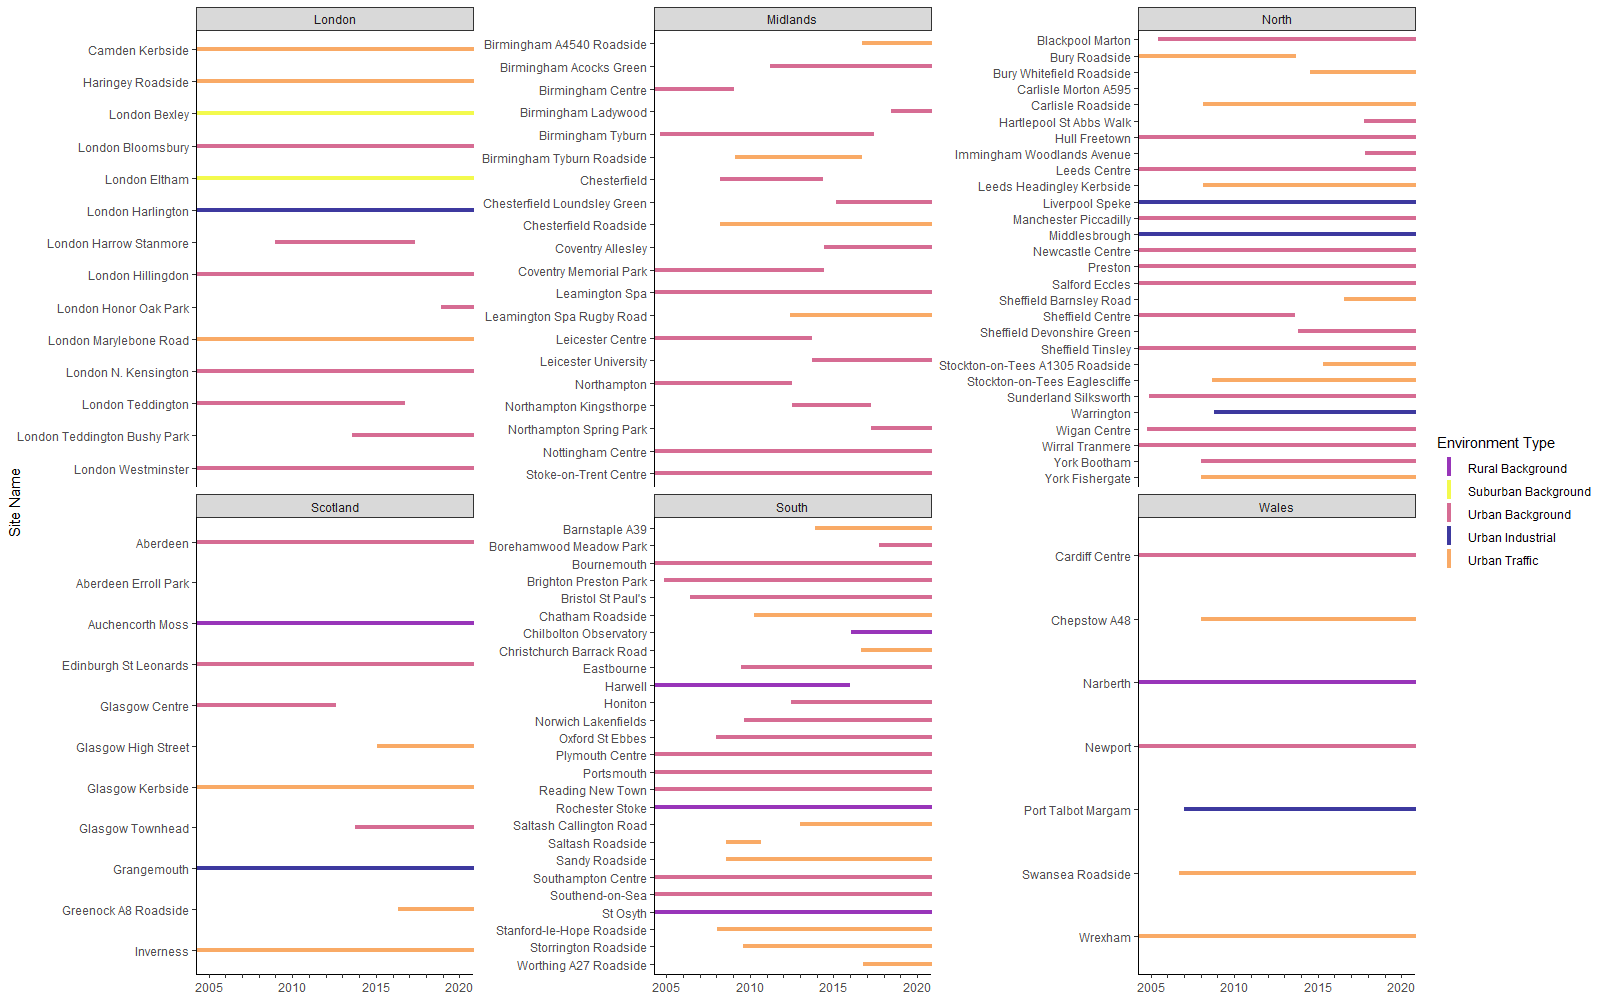
\includegraphics[width=1\textwidth]{Images/AURN Avaliability 2005-2020.png}
    \caption{Data Availability from AURN PM$_{2.5}$ Monitoring Sites 2005-2020}
    \label{fig:aurn}
\end{figure}

For PM2.5 the monthly mean is measured in $\mu g/m^3$ and aggregated from hourly measurements, with reported percentage of availability of data.

%https://uk-air.defra.gov.uk/assets/documents/reports/cat13/0902231025_VCM_Application_to_Hourly_and_AURN_FDMS_Purge_Measurements.pdf

Tapered Element Oscillating Microbalance
Beta Attenuation monitor
Gravimetric monitor
Filter Dynamics Measurement System (FDMS)
Optical light scattering
Fine Dust Analysis System (FIDAS)



\subsubsection{Satellite Data}
NASA's Moderate Resolution Imaging Spectroradiometer (MODIS) instrument operates on the Terra and Aqua satellites, each collecting daily data for 26 spectral wavelength bands. Estimating ground-level air quality and concentrations of pollutants relies on solar reflectance methods, primarily column-measured Aerosol Optical Depth (AOD) at 47 and 55 microns is used as a proxy measurement for PM$_{2.5}$ \citep{Christopher2010SatelliteProblem}. Many studies have been done to assess the accuracy and precision of approaches to estimating PM$_{2.5}$ ground concentrations from AOD \citep{Zhang2021SatellitePerspectives}, with time sequence algorithms such as NASA's multi-angle implementation of atmospheric correction (MAIAC) algorithm providing a significant improvement, as well as reprocessing to a finer grid. The MAIAC algorithm-based product (MCD19A2) is a Level 2 Gridded product produced daily from the Terra and Aqua MODIS inputs at a 1km pixel resolution, available for the entire study period.

The MAIAC algorithm is a reanalysis product from NASA of daily atmosphere and land surface, including AOD, cloud cover, column water vapour, and snow \citep{NASAMulti-AngleMCD19}. It is based on a sliding window technique of a time series using details about the surface and recent past observations to formulate and calibrate a daily global surface from 2000 to the present. This product was chosen due to past successes using the MAIAC adjusted AOD, such as in \cite{He2021TheAOD}, as well as, the spatial and temporal domains and resolutions lining up with the other modelling inputs. Furthermore, there is a concern when using raw or face value AOD for the UK, due to the persistent cloud cover over much of the UK across the year. 

The dataset was downloaded from NASA's Earth Data Search, for the swaths covering the UK (Swaths 16 and 17, see Figure \ref{fig:swaths}) for the period 2005 to 2020 at a daily resolution, there were 11,682 granules of data. 

\begin{figure}[h]
    \centering
    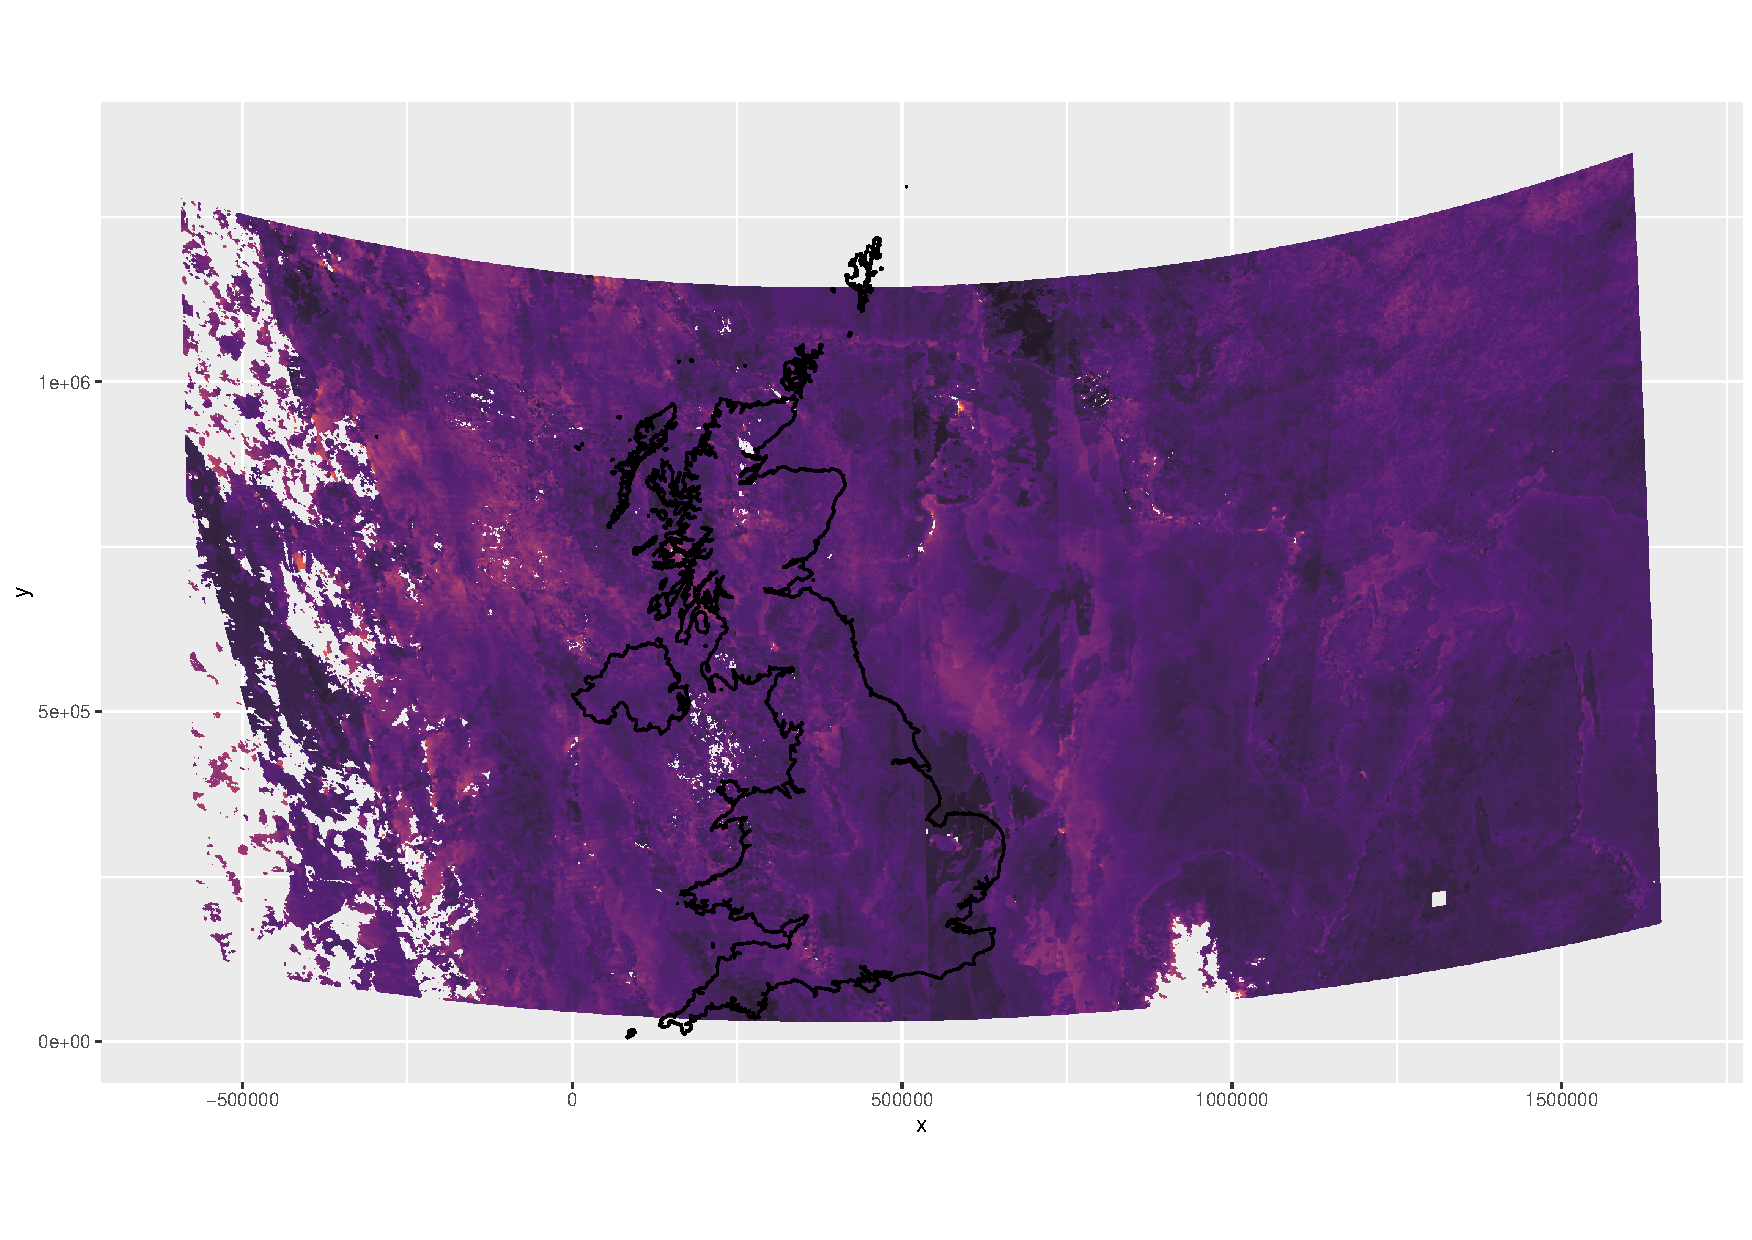
\includegraphics[width=1\textwidth]{Images/Swaths.pdf}
    \caption{Example of Swaths 16 and 17 from the MAIAC algorithm-derived AOD covering the UK: May 2018}
    \label{fig:swaths}
\end{figure}

%Aura OMI NO2 OMNO2d_HRM https://avdc.gsfc.nasa.gov/pub/data/satellite/Aura/OMI/V03/L3/OMNO2d_HR/

The data layers of interest are: Aerosol Optical Depth at 047 micron; Aerosol Optical Depth at 055 micron; and AOD Uncertainty at 047 micron.

\subsubsection{Underlying Model}
On review of the current underlying air pollution models for the UK, the Department for Environment, Food \& Rural Affairs' (Defra) Pollution Climate Mapping (PCM) model was selected for this study based on a number of different reasons. First, the modelling data is freely available, making reproduction of this study accessible and open source. Also, the PCM model is a background concentration model, meaning it can provide an additional layer to the overall model, instead of already being an approximation of actual pollution concentrations over the domain. Another requirement for the model choice was that it spans across the selected temporal domain, 2005-2020, for which the PCM model provides an annual mean concentration grid for Particulate Matter 2.5 (PM$_2.5$), Ozone (O$_3$), and Nitrogen Dioxide (NO$_2$), among others. Also importantly, the data is on a 1km x 1km grid for the entire UK, which is concordant with the other data sources and modelling choices. 

Finally, it was selected over the other commonly used UK Model, the Met Office's Air Quality in the Unified Model (AQUM) both due to spatial resolution and because of previous work by Forlani, showing a greater performance in a Bayesian spatiotemporal model when using the PCM model over AQUM for Greater London \cite{Forlani2020AR-INLA}.

The PCM model is a collection of multiple background and roadside air pollution models, produced to inform conformance to EU air pollution standards and regulations. The background concentrations for Nitrogen Oxides (NO$_x$) and Sulphur Dioxide (SO$_2$) are estimated from a wide range of air pollution dispersion and emission data, including from the Air Dispersion Model (ADMS) and the UK National Atmospheric Emission Inventory (NAEI). For PM$_2.5$ and PM$_10$, data for the variety of different constituents are estimated separately, for example, estimates for secondary inorganic aerosols come from interpolated measurements of SO$_4$, NO$_3$ and NH$_4$; secondary organic aerosol estimates are from the Numerical Atmospheric-dispersion Modelling Environment (NAME) model, and traffic related components are estimated from vehicle activity data and dispersion models. Nitrogen Dioxide (NO$_2$) and Ozone (O$_3$) background concentrations are then estimated through direct rural ground measurements and chemical equations of atmospheric reactions between pollutants, predominately using the relationship to NO$_x$. Further details of the modelling methods used are available from \cite{RicardoEnergyEnvironment2019Technical2019}. 

The downloaded data was available as one comma seperated value file per pollutant per year, with the data mapped onto the standard 1km x 1km BNG grid (see Figure \ref{fig:pcm}). The annual mean of PM$_{2.5}$ is recorded in $\mu g/m^3$.

\begin{figure}[h]
    \centering
    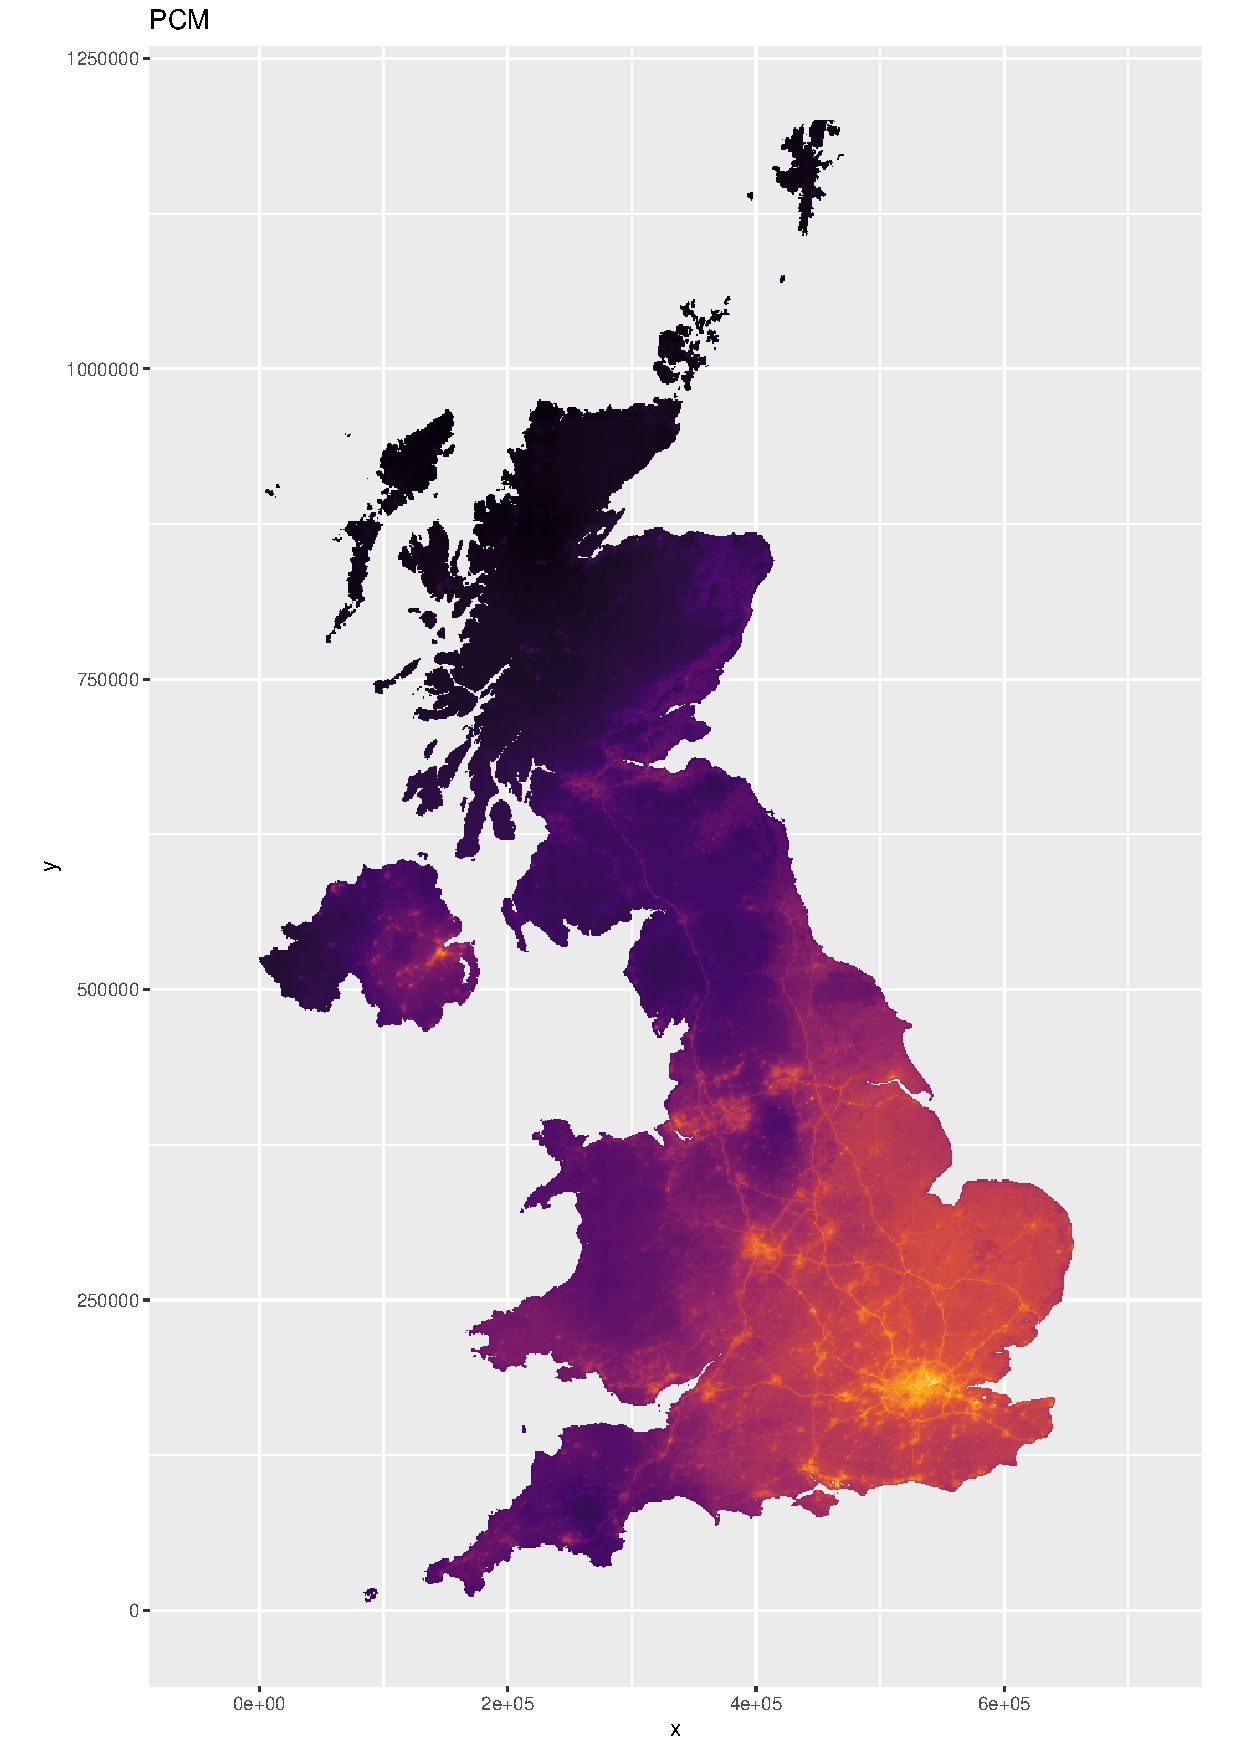
\includegraphics[width=0.4\textwidth]{Images/PCM.pdf}
    \caption{Example of UK Pollution Climate Mapping (PCM) Model: 2018}
    \label{fig:pcm}
\end{figure}

\subsubsection{Meteorological Data}
The ground level climate and meteorological observations for the UK are from the HadUK-Grid from the Met Office \citep{Hollis2019HadUK-GridAObservations}. It is a regressed interpolated grid of ground monitored weather observations, taking into account geographical location, terrain, land use and altitude, it is a relatively recent release by the Met Office and undergoes extensive quality control to increase accuracy and homogeneity away from monitoring sites. The downloaded dataset covers the UK at a 1km x 1km resolution BNG grid for 2005-2020, with a .nc file per variable per year for the monthly mean air temperature, total precipitation, and mean relative humidity (48 files in total, see Figure \ref{fig:met}). 

\begin{figure}[h]
    \centering
    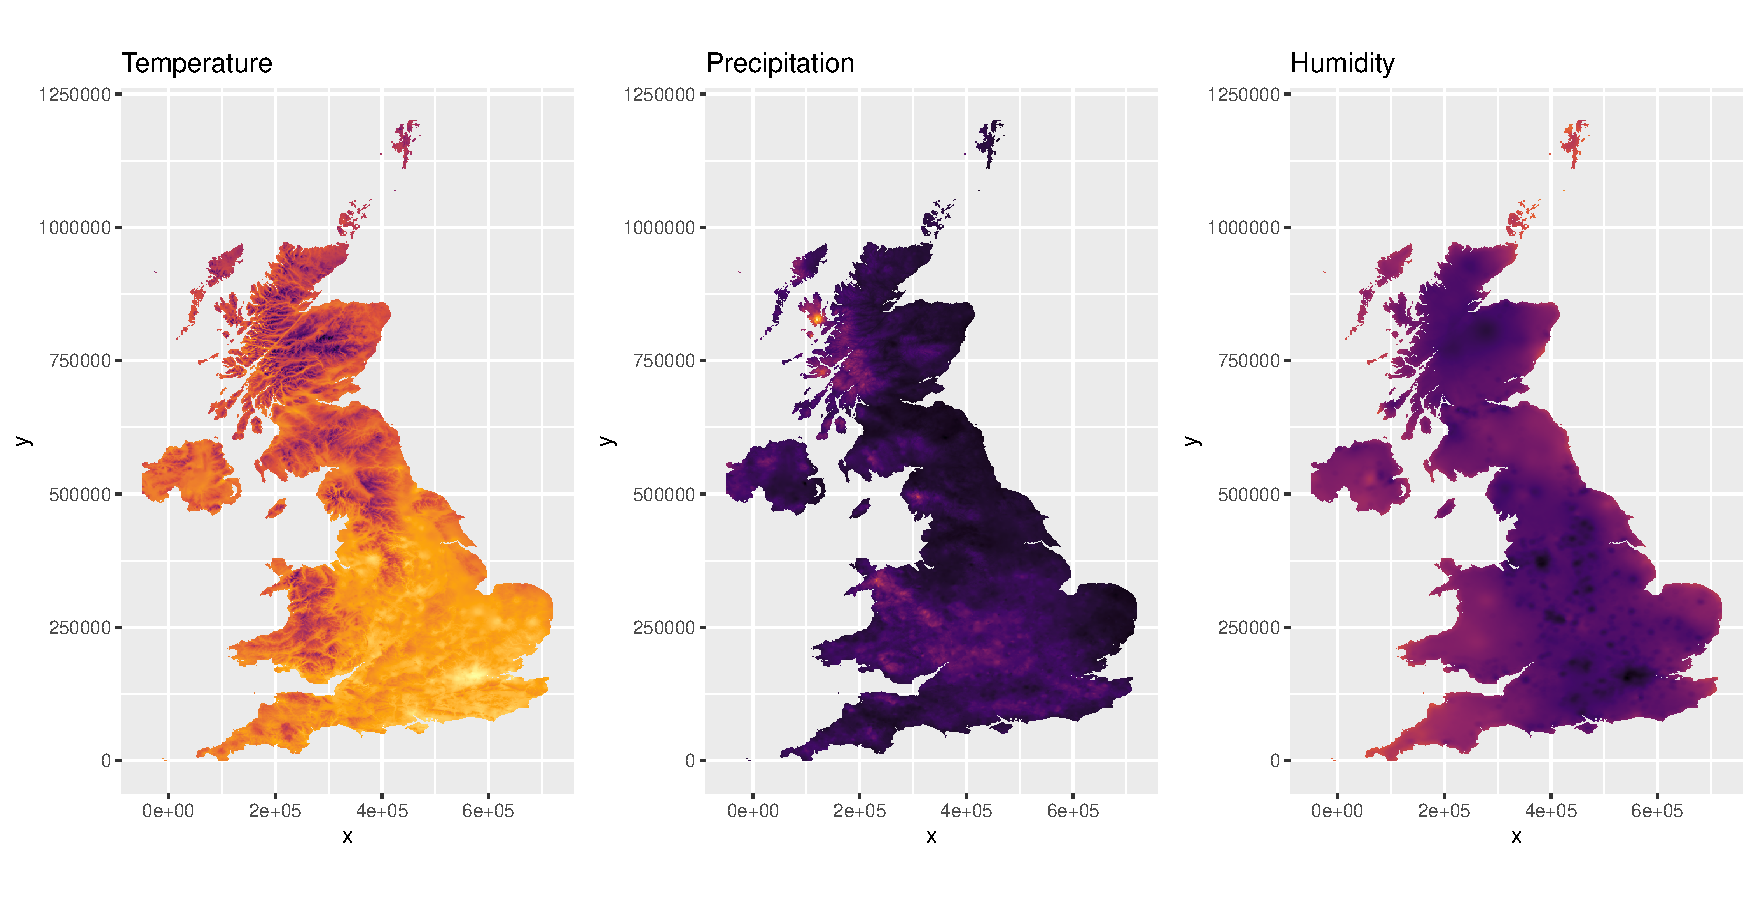
\includegraphics[width=1\textwidth]{Images/Met Data.pdf}
    \caption{Example of UK Meteorological Data for the HADUK-Grid: May 2018}
    \label{fig:met}
\end{figure}

\subsubsection{Boundary Layer Height}
Boundary Layer Height (BLH) is the height from the surface of the lowest layer of the atmosphere, in meters, and will be used in this application for the adjustment of satellite-derived AOD, as seen in \cite{He2019AGuangzhou}:
\begin{center}
    $AOD_{adjusted} = \frac{AOD_{observed}}{BLH}$
\end{center}
This is to approximate the relationship between the observed AOD and the true ground value. This data was downloaded from the European Centre for Medium-Range Weather Forecasts (ECMRWF) Reanalysis v5 (ERA5) database, available for the whole spatial and temporal domain as ... (type of file and for what?)


%\subsubsection{Population Data}
%Population Data

\subsection{Exposure Model}
Satellite data daily -> monthly
AQUM 1kmx1km? methods of misalignment (Chiara's paper ish)


DIAGRAM


London vs UK?

similar to \cite{deHoogh2018ModellingSwitzerland}
level 1: PM2.5/NO2 at monitoring stations 
level 2: PM2.5/NO2 at areas with AOD but no monitoring stations, 1kmx1km grid, methods of estimation/prediction from AOD
level 3: PM2.5/NO2 ar areas with no AOD or monitoring stations, 1kmx1km grid, interpolation of level 2, compare interpolation methods??? (ML, kriging, OI, etc)

UPDATED:
level 1: PM2.5/NO2 at monitoring stations 
level 2: PM2.5/NO2 interpolated AOD but no monitoring stations, 1kmx1km grid, compare interpolation methods??? (ML, kriging, OI, etc)
level 3: PM2.5/NO2 at areas with no monitoring stations from AOD and other variables, 1kmx1km grid

%from poster

Using a 3-staged modelling approach to model PM$_{2.5}$ concentrations across the UK, in a similar way to \cite{Kloog2014AData}:

\textbf{Stage 1}: Interpolate satellite derived aerosol optical depth to entire study domain, comparing 3 main spatiotemporal interpolation methods \citep{Susanto2016SpatiotemporalModelling}:
\begin{itemize}
    \item Inverse Distance Weighting (IDW)
    \item Ordinary Kriging (OK)
    \item Random Forest (RF)
\end{itemize}
%could also do Nearest Neighbour and Neural Networks???

\textbf{Stage 2}: 
Fit a hierarchical Bayesian geostatistical spatio-temporal regression model at the monitoring station sites:
\cite[p.459-461]{Gelfand2019HandbookStatistics}

Option 1: Spatial Downscaler
Assume ground monitoring is the true values\\
$ Y(\textbf{s},t) = \beta(\textbf{s},t) \textbf{X}(\textbf{s},t)  + e(\textbf{s},t) $\\
$ e(\textbf{s},t) = \omega(\textbf{s},t)  + \varepsilon(\textbf{s},t) $ \\
\begin{itemize}
 \item $Y(\textbf{s},t)$ concentration at location \textbf{s}, time t
 \item $\textbf{X}(\textbf{s},t)$ temperature, precipitation, humidity, PCM, AOD and population covariates at location \textbf{s}, time t with coefficients $\beta(\textbf{s},t)$
 \item $\omega(\textbf{s},t)$ spatiotemporal random effect term
 \item $\varepsilon(\textbf{s},t)$ mean zero spatiotemporal Gaussian process error term
\end{itemize}
%For the spatiotemporal random effect term, $\omega(\textbf{s},t)$, we considered 3 forms: \\
 %$\omega(\textbf{s},t)  = \alpha(t)  + \omega(\textbf{s}), \alpha(t+1) = \rho \alpha(t) + \eta(t), \eta(t) \sim \mathcal{N}(0,\sigma_{\alpha}^2) $ \\
 %$\omega(\textbf{s},t)  = \alpha_{\textbf{s}}(t) $\\
 %$\omega(\textbf{s},t)  = \omega_{t}(\textbf{s}) $

Option 2: Spatial Bayesian Melding
Assume another underlying process Z \\
$ Y(\textbf{s},t) = \textbf{Z}(\textbf{s},t)  + e_F(\textbf{s},t) $\\
$ \tilde{Y}(\textbf{s},t) = \alpha(\textbf{s},t) \textbf{X}(\textbf{s},t) + e_N(\textbf{s},t) $\\
$ Z(\textbf{s},t) = \beta(\textbf{s},t) \textbf{M}(\textbf{s},t)  + e_z(\textbf{s},t) $\\
$ e_z(\textbf{s},t) = \omega(\textbf{s},t)  + \varepsilon(\textbf{s},t) $ \\
\begin{itemize}
 \item $Y(\textbf{s},t)$ concentration at location \textbf{s}, time t
 \item $\tilde{Y}(\textbf{s},t)$ estimated concentration at location \textbf{s}, time t
 \item $Z(\textbf{s},t)$ true underlying spatio-temporal process at location \textbf{s}, time t
  \item $\textbf{X}(\textbf{s},t)$ ground monitored data, PCM and AOD at location \textbf{s}, time t with coefficients $\beta(\textbf{s},t)$
 \item $\textbf{M}(\textbf{s},t)$ temperature, precipitation, humidity, and population covariates at location \textbf{s}, time t with coefficients $\beta(\textbf{s},t)$
 \item $e_F(\textbf{s},t)$ measurement error term
 \item $e_N(\textbf{s},t)$ ??? error term
 \item $\omega(\textbf{s},t)$ spatiotemporal random effect term
 \item $\varepsilon(\textbf{s},t)$ mean zero spatiotemporal Gaussian process error term
\end{itemize}

BAYESIAN MELDING IS COMPUTATIONALLY EXPENSIVE, MAYBE JUST INCLUDE MEASUREMENTS ERRORS OR FUTURUE APPROACH


\textbf{Stage 3}: Estimate PM$_{2.5}$ at locations and times across whole domain, using stage 1, AOD, metero, etc
$f(Y((\textbf{s}_0,t_0)|\textbf{Y})$
for all unmonitored locations $\textbf{s}_0$ at times $t_0$ in study domain.


%%imput AOD through underlying model???

%use population as weights??

boundaries and extremes: important? link to biobank?


\section{Current Progress}

Current work so far: analysis, models, graphs, data applications

The preliminary stages of this objective involved development of the skills in this area of modelling (see Section \ref{Sec: Dev}), acquiring and processing the air pollution and related datasets (see Appendix \ref{App:Preprocessing}), and some preliminary analysis of the data (see Appendix \ref{App:preanalysis}). The techniques and insights developed from these stages of research have influenced and complemented the approach to the overall exposure modelling.

\section{Spatial Models} \label{Spatial}
 - Spatial interpolation May 2018
 - London model May 2018
 - UK model May 2018
 
 
\subsection{London Spatial-temporal Model}
Limiting the spatial domain to a bounding box of Greater London provides a starting point for developing the whole exposure model, this reduces the dimensionality of the data and enables the use of the stationarity assumption. Stationarity of spatial processes assumes that the distribution of the spatial process is constant over translation, i.e. "for any given $n \geq 1$, any set of $n$ sites $\{s_1,...,s_n\}$ and any $h \in \mathbb{R}$, the distribution of $(Y(s_1),...,Y(s_n))$ is the same as that of $(Y(s_1+h),...,Y(s_n+h))$" \citep[p.23-24]{Banerjee2014}. Greater London also has a very high density of ground monitoring stations for reduced uncertainity in the model, and more existing similar exposure models, such as \cite{Forlani2020AR-INLA}, for model comparison.

As per the outlined methods, the first stage of the exposure model is the interpolation of the satellite-derived aerosol optical depth across the whole space and time domains. Three commonly used interpolation methods are used: Inverse Distance Weighting (IDW), Ordinary Kriging (OK), and Random Forest (RF). The R code for fitting, modelling and cross-validation is in the GitHub repository in Appendix \ref{GitHub}, and Figure \ref{fig:AODinter} shows the resulting surfaces for .... (a couple of different months pls).

\begin{figure}[h]
    \centering
    \includegraphics[width=1\textwidth]{...}
    \caption{Interpolation AOD surfaces for ...}
    \label{fig:AODinter}
\end{figure}

Cross-validation results...

 - Interpolate AOD, cross-validation?
 - Model
 - Code/packages
 - Model parameters and tuning
 - Cross Validation

\section{Next Steps}
- Further testing/cross validation of london?
- UK model
- outputs???
- visualisation
